% Generated by Sphinx.
\def\sphinxdocclass{report}
\documentclass[letterpaper,10pt,english]{sphinxmanual}
\usepackage[utf8]{inputenc}
\DeclareUnicodeCharacter{00A0}{\nobreakspace}
\usepackage[T1]{fontenc}
\usepackage{babel}
\usepackage{times}
\usepackage[Bjarne]{fncychap}
\usepackage{longtable}
\usepackage{sphinx}
\usepackage{multirow}


\title{Model Checking for tcc Calculus Documentation}
\date{November 15, 2012}
\release{1.0}
\author{Jaime E. Arias Almeida}
\newcommand{\sphinxlogo}{}
\renewcommand{\releasename}{Release}
\makeindex

\makeatletter
\def\PYG@reset{\let\PYG@it=\relax \let\PYG@bf=\relax%
    \let\PYG@ul=\relax \let\PYG@tc=\relax%
    \let\PYG@bc=\relax \let\PYG@ff=\relax}
\def\PYG@tok#1{\csname PYG@tok@#1\endcsname}
\def\PYG@toks#1+{\ifx\relax#1\empty\else%
    \PYG@tok{#1}\expandafter\PYG@toks\fi}
\def\PYG@do#1{\PYG@bc{\PYG@tc{\PYG@ul{%
    \PYG@it{\PYG@bf{\PYG@ff{#1}}}}}}}
\def\PYG#1#2{\PYG@reset\PYG@toks#1+\relax+\PYG@do{#2}}

\expandafter\def\csname PYG@tok@gd\endcsname{\def\PYG@tc##1{\textcolor[rgb]{0.63,0.00,0.00}{##1}}}
\expandafter\def\csname PYG@tok@gu\endcsname{\let\PYG@bf=\textbf\def\PYG@tc##1{\textcolor[rgb]{0.50,0.00,0.50}{##1}}}
\expandafter\def\csname PYG@tok@gt\endcsname{\def\PYG@tc##1{\textcolor[rgb]{0.00,0.25,0.82}{##1}}}
\expandafter\def\csname PYG@tok@gs\endcsname{\let\PYG@bf=\textbf}
\expandafter\def\csname PYG@tok@gr\endcsname{\def\PYG@tc##1{\textcolor[rgb]{1.00,0.00,0.00}{##1}}}
\expandafter\def\csname PYG@tok@cm\endcsname{\let\PYG@it=\textit\def\PYG@tc##1{\textcolor[rgb]{0.25,0.50,0.56}{##1}}}
\expandafter\def\csname PYG@tok@vg\endcsname{\def\PYG@tc##1{\textcolor[rgb]{0.73,0.38,0.84}{##1}}}
\expandafter\def\csname PYG@tok@m\endcsname{\def\PYG@tc##1{\textcolor[rgb]{0.13,0.50,0.31}{##1}}}
\expandafter\def\csname PYG@tok@mh\endcsname{\def\PYG@tc##1{\textcolor[rgb]{0.13,0.50,0.31}{##1}}}
\expandafter\def\csname PYG@tok@cs\endcsname{\def\PYG@tc##1{\textcolor[rgb]{0.25,0.50,0.56}{##1}}\def\PYG@bc##1{\setlength{\fboxsep}{0pt}\colorbox[rgb]{1.00,0.94,0.94}{\strut ##1}}}
\expandafter\def\csname PYG@tok@ge\endcsname{\let\PYG@it=\textit}
\expandafter\def\csname PYG@tok@vc\endcsname{\def\PYG@tc##1{\textcolor[rgb]{0.73,0.38,0.84}{##1}}}
\expandafter\def\csname PYG@tok@il\endcsname{\def\PYG@tc##1{\textcolor[rgb]{0.13,0.50,0.31}{##1}}}
\expandafter\def\csname PYG@tok@go\endcsname{\def\PYG@tc##1{\textcolor[rgb]{0.19,0.19,0.19}{##1}}}
\expandafter\def\csname PYG@tok@cp\endcsname{\def\PYG@tc##1{\textcolor[rgb]{0.00,0.44,0.13}{##1}}}
\expandafter\def\csname PYG@tok@gi\endcsname{\def\PYG@tc##1{\textcolor[rgb]{0.00,0.63,0.00}{##1}}}
\expandafter\def\csname PYG@tok@gh\endcsname{\let\PYG@bf=\textbf\def\PYG@tc##1{\textcolor[rgb]{0.00,0.00,0.50}{##1}}}
\expandafter\def\csname PYG@tok@ni\endcsname{\let\PYG@bf=\textbf\def\PYG@tc##1{\textcolor[rgb]{0.84,0.33,0.22}{##1}}}
\expandafter\def\csname PYG@tok@nl\endcsname{\let\PYG@bf=\textbf\def\PYG@tc##1{\textcolor[rgb]{0.00,0.13,0.44}{##1}}}
\expandafter\def\csname PYG@tok@nn\endcsname{\let\PYG@bf=\textbf\def\PYG@tc##1{\textcolor[rgb]{0.05,0.52,0.71}{##1}}}
\expandafter\def\csname PYG@tok@no\endcsname{\def\PYG@tc##1{\textcolor[rgb]{0.38,0.68,0.84}{##1}}}
\expandafter\def\csname PYG@tok@na\endcsname{\def\PYG@tc##1{\textcolor[rgb]{0.25,0.44,0.63}{##1}}}
\expandafter\def\csname PYG@tok@nb\endcsname{\def\PYG@tc##1{\textcolor[rgb]{0.00,0.44,0.13}{##1}}}
\expandafter\def\csname PYG@tok@nc\endcsname{\let\PYG@bf=\textbf\def\PYG@tc##1{\textcolor[rgb]{0.05,0.52,0.71}{##1}}}
\expandafter\def\csname PYG@tok@nd\endcsname{\let\PYG@bf=\textbf\def\PYG@tc##1{\textcolor[rgb]{0.33,0.33,0.33}{##1}}}
\expandafter\def\csname PYG@tok@ne\endcsname{\def\PYG@tc##1{\textcolor[rgb]{0.00,0.44,0.13}{##1}}}
\expandafter\def\csname PYG@tok@nf\endcsname{\def\PYG@tc##1{\textcolor[rgb]{0.02,0.16,0.49}{##1}}}
\expandafter\def\csname PYG@tok@si\endcsname{\let\PYG@it=\textit\def\PYG@tc##1{\textcolor[rgb]{0.44,0.63,0.82}{##1}}}
\expandafter\def\csname PYG@tok@s2\endcsname{\def\PYG@tc##1{\textcolor[rgb]{0.25,0.44,0.63}{##1}}}
\expandafter\def\csname PYG@tok@vi\endcsname{\def\PYG@tc##1{\textcolor[rgb]{0.73,0.38,0.84}{##1}}}
\expandafter\def\csname PYG@tok@nt\endcsname{\let\PYG@bf=\textbf\def\PYG@tc##1{\textcolor[rgb]{0.02,0.16,0.45}{##1}}}
\expandafter\def\csname PYG@tok@nv\endcsname{\def\PYG@tc##1{\textcolor[rgb]{0.73,0.38,0.84}{##1}}}
\expandafter\def\csname PYG@tok@s1\endcsname{\def\PYG@tc##1{\textcolor[rgb]{0.25,0.44,0.63}{##1}}}
\expandafter\def\csname PYG@tok@gp\endcsname{\let\PYG@bf=\textbf\def\PYG@tc##1{\textcolor[rgb]{0.78,0.36,0.04}{##1}}}
\expandafter\def\csname PYG@tok@sh\endcsname{\def\PYG@tc##1{\textcolor[rgb]{0.25,0.44,0.63}{##1}}}
\expandafter\def\csname PYG@tok@ow\endcsname{\let\PYG@bf=\textbf\def\PYG@tc##1{\textcolor[rgb]{0.00,0.44,0.13}{##1}}}
\expandafter\def\csname PYG@tok@sx\endcsname{\def\PYG@tc##1{\textcolor[rgb]{0.78,0.36,0.04}{##1}}}
\expandafter\def\csname PYG@tok@bp\endcsname{\def\PYG@tc##1{\textcolor[rgb]{0.00,0.44,0.13}{##1}}}
\expandafter\def\csname PYG@tok@c1\endcsname{\let\PYG@it=\textit\def\PYG@tc##1{\textcolor[rgb]{0.25,0.50,0.56}{##1}}}
\expandafter\def\csname PYG@tok@kc\endcsname{\let\PYG@bf=\textbf\def\PYG@tc##1{\textcolor[rgb]{0.00,0.44,0.13}{##1}}}
\expandafter\def\csname PYG@tok@c\endcsname{\let\PYG@it=\textit\def\PYG@tc##1{\textcolor[rgb]{0.25,0.50,0.56}{##1}}}
\expandafter\def\csname PYG@tok@mf\endcsname{\def\PYG@tc##1{\textcolor[rgb]{0.13,0.50,0.31}{##1}}}
\expandafter\def\csname PYG@tok@err\endcsname{\def\PYG@bc##1{\setlength{\fboxsep}{0pt}\fcolorbox[rgb]{1.00,0.00,0.00}{1,1,1}{\strut ##1}}}
\expandafter\def\csname PYG@tok@kd\endcsname{\let\PYG@bf=\textbf\def\PYG@tc##1{\textcolor[rgb]{0.00,0.44,0.13}{##1}}}
\expandafter\def\csname PYG@tok@ss\endcsname{\def\PYG@tc##1{\textcolor[rgb]{0.32,0.47,0.09}{##1}}}
\expandafter\def\csname PYG@tok@sr\endcsname{\def\PYG@tc##1{\textcolor[rgb]{0.14,0.33,0.53}{##1}}}
\expandafter\def\csname PYG@tok@mo\endcsname{\def\PYG@tc##1{\textcolor[rgb]{0.13,0.50,0.31}{##1}}}
\expandafter\def\csname PYG@tok@mi\endcsname{\def\PYG@tc##1{\textcolor[rgb]{0.13,0.50,0.31}{##1}}}
\expandafter\def\csname PYG@tok@kn\endcsname{\let\PYG@bf=\textbf\def\PYG@tc##1{\textcolor[rgb]{0.00,0.44,0.13}{##1}}}
\expandafter\def\csname PYG@tok@o\endcsname{\def\PYG@tc##1{\textcolor[rgb]{0.40,0.40,0.40}{##1}}}
\expandafter\def\csname PYG@tok@kr\endcsname{\let\PYG@bf=\textbf\def\PYG@tc##1{\textcolor[rgb]{0.00,0.44,0.13}{##1}}}
\expandafter\def\csname PYG@tok@s\endcsname{\def\PYG@tc##1{\textcolor[rgb]{0.25,0.44,0.63}{##1}}}
\expandafter\def\csname PYG@tok@kp\endcsname{\def\PYG@tc##1{\textcolor[rgb]{0.00,0.44,0.13}{##1}}}
\expandafter\def\csname PYG@tok@w\endcsname{\def\PYG@tc##1{\textcolor[rgb]{0.73,0.73,0.73}{##1}}}
\expandafter\def\csname PYG@tok@kt\endcsname{\def\PYG@tc##1{\textcolor[rgb]{0.56,0.13,0.00}{##1}}}
\expandafter\def\csname PYG@tok@sc\endcsname{\def\PYG@tc##1{\textcolor[rgb]{0.25,0.44,0.63}{##1}}}
\expandafter\def\csname PYG@tok@sb\endcsname{\def\PYG@tc##1{\textcolor[rgb]{0.25,0.44,0.63}{##1}}}
\expandafter\def\csname PYG@tok@k\endcsname{\let\PYG@bf=\textbf\def\PYG@tc##1{\textcolor[rgb]{0.00,0.44,0.13}{##1}}}
\expandafter\def\csname PYG@tok@se\endcsname{\let\PYG@bf=\textbf\def\PYG@tc##1{\textcolor[rgb]{0.25,0.44,0.63}{##1}}}
\expandafter\def\csname PYG@tok@sd\endcsname{\let\PYG@it=\textit\def\PYG@tc##1{\textcolor[rgb]{0.25,0.44,0.63}{##1}}}

\def\PYGZbs{\char`\\}
\def\PYGZus{\char`\_}
\def\PYGZob{\char`\{}
\def\PYGZcb{\char`\}}
\def\PYGZca{\char`\^}
\def\PYGZam{\char`\&}
\def\PYGZlt{\char`\<}
\def\PYGZgt{\char`\>}
\def\PYGZsh{\char`\#}
\def\PYGZpc{\char`\%}
\def\PYGZdl{\char`\$}
\def\PYGZti{\char`\~}
% for compatibility with earlier versions
\def\PYGZat{@}
\def\PYGZlb{[}
\def\PYGZrb{]}
\makeatother

\begin{document}

\maketitle
\tableofcontents
\phantomsection\label{index::doc}


Contents:


\chapter{Formula}
\label{formula:formula}\label{formula:module-formula}\label{formula::doc}\label{formula:welcome-to-model-checking-for-tcc-calculus-s-documentation}\index{formula (module)}
This module contains the class to describe a temporal formula.
\index{Formula (class in formula)}

\begin{fulllineitems}
\phantomsection\label{formula:formula.Formula}\pysiglinewithargsret{\strong{class }\code{formula.}\bfcode{Formula}}{\emph{data}}{}
This class represents a temporal formula.
\begin{quote}\begin{description}
\item[{Parameters}] \leavevmode
\textbf{data} (\emph{Dictionary.}) -- Structure representing the temporal formula.

\item[{Example }] \leavevmode
\end{description}\end{quote}

$\phi = \diamondsuit(\mathtt{in=true} \wedge \neg\circ(\mathtt{x=2}))$

\begin{Verbatim}[commandchars=\\\{\}]
\PYG{g+gp}{\PYGZgt{}\PYGZgt{}\PYGZgt{} }\PYG{k+kn}{from} \PYG{n+nn}{formula} \PYG{k+kn}{import} \PYG{o}{*}
\PYG{g+gp}{\PYGZgt{}\PYGZgt{}\PYGZgt{} }\PYG{n}{phi} \PYG{o}{=} \PYG{n}{Formula}\PYG{p}{(}\PYG{p}{\PYGZob{}}\PYG{l+s}{"}\PYG{l+s}{\PYGZlt{}\PYGZgt{}}\PYG{l+s}{"}\PYG{p}{:} \PYG{p}{\PYGZob{}}\PYG{l+s}{"}\PYG{l+s}{\PYGZca{}}\PYG{l+s}{"}\PYG{p}{:}\PYG{p}{\PYGZob{}}\PYG{l+s}{"}\PYG{l+s}{"}\PYG{p}{:}\PYG{l+s}{"}\PYG{l+s}{in=true}\PYG{l+s}{"}\PYG{p}{,}\PYG{l+s}{"}\PYG{l+s}{\PYGZti{}}\PYG{l+s}{"}\PYG{p}{:}\PYG{p}{\PYGZob{}}\PYG{l+s}{"}\PYG{l+s}{o}\PYG{l+s}{"}\PYG{p}{:}\PYG{l+s}{"}\PYG{l+s}{x=2}\PYG{l+s}{"}\PYG{p}{\PYGZcb{}}\PYG{p}{\PYGZcb{}}\PYG{p}{\PYGZcb{}}\PYG{p}{\PYGZcb{}}\PYG{p}{)}
\end{Verbatim}

\begin{notice}{note}{Note:}
Logic operators are represented by the following symbols:
\begin{itemize}
\item {} 
Globally : \code{{[}{]}}

\item {} 
Future : \code{\textless{}\textgreater{}}

\item {} 
Next : \code{o}

\item {} 
Negation : \code{\textasciitilde{}}

\item {} 
Or : \code{v}

\item {} 
And : \code{\textasciicircum{}}

\end{itemize}
\end{notice}
\index{getConnective() (formula.Formula method)}

\begin{fulllineitems}
\phantomsection\label{formula:formula.Formula.getConnective}\pysiglinewithargsret{\bfcode{getConnective}}{}{}
Return the main connective of the formula.
\begin{quote}\begin{description}
\item[{Returns}] \leavevmode
A string representing the main connective of the formula.

\item[{Return type}] \leavevmode
String.

\item[{Example }] \leavevmode
\end{description}\end{quote}

$\phi = \diamondsuit(\mathtt{in=true} \wedge \neg\circ(\mathtt{x=2})) \hspace{2cm} getConnective(\phi) = \diamondsuit$

\begin{Verbatim}[commandchars=\\\{\}]
\PYG{g+gp}{\PYGZgt{}\PYGZgt{}\PYGZgt{} }\PYG{k+kn}{from} \PYG{n+nn}{formula} \PYG{k+kn}{import} \PYG{o}{*}
\PYG{g+gp}{\PYGZgt{}\PYGZgt{}\PYGZgt{} }\PYG{n}{phi} \PYG{o}{=} \PYG{n}{Formula}\PYG{p}{(}\PYG{p}{\PYGZob{}}\PYG{l+s}{"}\PYG{l+s}{\PYGZlt{}\PYGZgt{}}\PYG{l+s}{"}\PYG{p}{:} \PYG{p}{\PYGZob{}}\PYG{l+s}{"}\PYG{l+s}{\PYGZca{}}\PYG{l+s}{"}\PYG{p}{:}\PYG{p}{\PYGZob{}}\PYG{l+s}{"}\PYG{l+s}{"}\PYG{p}{:}\PYG{l+s}{"}\PYG{l+s}{in=true}\PYG{l+s}{"}\PYG{p}{,}\PYG{l+s}{"}\PYG{l+s}{\PYGZti{}}\PYG{l+s}{"}\PYG{p}{:}\PYG{p}{\PYGZob{}}\PYG{l+s}{"}\PYG{l+s}{o}\PYG{l+s}{"}\PYG{p}{:}\PYG{l+s}{"}\PYG{l+s}{x=2}\PYG{l+s}{"}\PYG{p}{\PYGZcb{}}\PYG{p}{\PYGZcb{}}\PYG{p}{\PYGZcb{}}\PYG{p}{\PYGZcb{}}\PYG{p}{)}
\PYG{g+gp}{\PYGZgt{}\PYGZgt{}\PYGZgt{} }\PYG{n}{phi}\PYG{o}{.}\PYG{n}{getConnective}\PYG{p}{(}\PYG{p}{)}
\PYG{g+go}{'\PYGZlt{}\PYGZgt{}'}
\end{Verbatim}

\end{fulllineitems}

\index{getConsistentPropositions() (formula.Formula method)}

\begin{fulllineitems}
\phantomsection\label{formula:formula.Formula.getConsistentPropositions}\pysiglinewithargsret{\bfcode{getConsistentPropositions}}{}{}
Returns the consistent propositions of a formula.
\begin{quote}\begin{description}
\item[{Returns}] \leavevmode
A structure representing the consistent proposition of the formula.

\item[{Return type}] \leavevmode
Dictionary.

\item[{Example }] \leavevmode
\end{description}\end{quote}

$\phi = (x = 2) \hspace{2cm} consistentPropositions(\phi) = \neg(x=1)$

\begin{Verbatim}[commandchars=\\\{\}]
\PYG{g+gp}{\PYGZgt{}\PYGZgt{}\PYGZgt{} }\PYG{k+kn}{from} \PYG{n+nn}{formula} \PYG{k+kn}{import} \PYG{o}{*}
\PYG{g+gp}{\PYGZgt{}\PYGZgt{}\PYGZgt{} }\PYG{n}{phi} \PYG{o}{=} \PYG{n}{Formula}\PYG{p}{(}\PYG{p}{\PYGZob{}}\PYG{l+s}{"}\PYG{l+s}{"}\PYG{p}{:} \PYG{l+s}{"}\PYG{l+s}{x=2}\PYG{l+s}{"}\PYG{p}{\PYGZcb{}}\PYG{p}{)}
\PYG{g+gp}{\PYGZgt{}\PYGZgt{}\PYGZgt{} }\PYG{n}{phi}\PYG{o}{.}\PYG{n}{getConsistentPropositions}\PYG{p}{(}\PYG{p}{)}
\PYG{g+go}{\PYGZob{}'\PYGZti{}': 'x=1'\PYGZcb{}}
\end{Verbatim}

\end{fulllineitems}

\index{getFormula() (formula.Formula method)}

\begin{fulllineitems}
\phantomsection\label{formula:formula.Formula.getFormula}\pysiglinewithargsret{\bfcode{getFormula}}{}{}
Returns the formula.
\begin{quote}\begin{description}
\item[{Returns}] \leavevmode
A structure representing the formula.

\item[{Return type}] \leavevmode
Dictionary.

\item[{Example }] \leavevmode
\end{description}\end{quote}

\begin{Verbatim}[commandchars=\\\{\}]
\PYG{g+gp}{\PYGZgt{}\PYGZgt{}\PYGZgt{} }\PYG{k+kn}{from} \PYG{n+nn}{formula} \PYG{k+kn}{import} \PYG{o}{*}
\PYG{g+gp}{\PYGZgt{}\PYGZgt{}\PYGZgt{} }\PYG{n}{phi} \PYG{o}{=} \PYG{n}{Formula}\PYG{p}{(}\PYG{p}{\PYGZob{}}\PYG{l+s}{"}\PYG{l+s}{\PYGZlt{}\PYGZgt{}}\PYG{l+s}{"}\PYG{p}{:} \PYG{p}{\PYGZob{}}\PYG{l+s}{"}\PYG{l+s}{\PYGZca{}}\PYG{l+s}{"}\PYG{p}{:}\PYG{p}{\PYGZob{}}\PYG{l+s}{"}\PYG{l+s}{"}\PYG{p}{:}\PYG{l+s}{"}\PYG{l+s}{in=true}\PYG{l+s}{"}\PYG{p}{,}\PYG{l+s}{"}\PYG{l+s}{\PYGZti{}}\PYG{l+s}{"}\PYG{p}{:}\PYG{p}{\PYGZob{}}\PYG{l+s}{"}\PYG{l+s}{o}\PYG{l+s}{"}\PYG{p}{:}\PYG{l+s}{"}\PYG{l+s}{x=2}\PYG{l+s}{"}\PYG{p}{\PYGZcb{}}\PYG{p}{\PYGZcb{}}\PYG{p}{\PYGZcb{}}\PYG{p}{\PYGZcb{}}\PYG{p}{)}
\PYG{g+gp}{\PYGZgt{}\PYGZgt{}\PYGZgt{} }\PYG{n}{phi}\PYG{o}{.}\PYG{n}{getFormula}\PYG{p}{(}\PYG{p}{)}
\PYG{g+go}{\PYGZob{}'\PYGZlt{}\PYGZgt{}': \PYGZob{}'\PYGZca{}': \PYGZob{}'': 'in=true', '\PYGZti{}': \PYGZob{}'o': 'x=2'\PYGZcb{}\PYGZcb{}\PYGZcb{}\PYGZcb{}}
\end{Verbatim}

\end{fulllineitems}

\index{getNegation() (formula.Formula method)}

\begin{fulllineitems}
\phantomsection\label{formula:formula.Formula.getNegation}\pysiglinewithargsret{\bfcode{getNegation}}{}{}
Returns the negation of the formula.
\begin{quote}\begin{description}
\item[{Returns}] \leavevmode
The negation of the formula.

\item[{Return type}] \leavevmode
{\hyperref[formula:formula.Formula]{\code{Formula}}}.

\item[{Example }] \leavevmode
\end{description}\end{quote}

$\phi = \circ(\mathtt{x=2}) \hspace{2cm} \neg\phi = \neg\circ(\mathtt{x=2})$

\begin{Verbatim}[commandchars=\\\{\}]
\PYG{g+gp}{\PYGZgt{}\PYGZgt{}\PYGZgt{} }\PYG{k+kn}{from} \PYG{n+nn}{formula} \PYG{k+kn}{import} \PYG{o}{*}
\PYG{g+gp}{\PYGZgt{}\PYGZgt{}\PYGZgt{} }\PYG{n}{phi} \PYG{o}{=} \PYG{n}{Formula}\PYG{p}{(}\PYG{p}{\PYGZob{}}\PYG{l+s}{"}\PYG{l+s}{o}\PYG{l+s}{"}\PYG{p}{:}\PYG{l+s}{"}\PYG{l+s}{x=2}\PYG{l+s}{"}\PYG{p}{\PYGZcb{}}\PYG{p}{)}
\PYG{g+gp}{\PYGZgt{}\PYGZgt{}\PYGZgt{} }\PYG{n}{negPhi} \PYG{o}{=} \PYG{n}{phi}\PYG{o}{.}\PYG{n}{getNegation}\PYG{p}{(}\PYG{p}{)}
\PYG{g+gp}{\PYGZgt{}\PYGZgt{}\PYGZgt{} }\PYG{n}{negPhi}\PYG{o}{.}\PYG{n}{getFormula}\PYG{p}{(}\PYG{p}{)}
\PYG{g+go}{\PYGZob{}'\PYGZti{}': \PYGZob{}'o': 'x=2'\PYGZcb{}\PYGZcb{}}
\end{Verbatim}

\end{fulllineitems}

\index{getPropositionRules() (formula.Formula method)}

\begin{fulllineitems}
\phantomsection\label{formula:formula.Formula.getPropositionRules}\pysiglinewithargsret{\bfcode{getPropositionRules}}{}{}
Returns the consistent propositions of all propositions in the implementation.
\begin{quote}\begin{description}
\item[{Example }] \leavevmode
\item[{Returns}] \leavevmode
A dictionary containing as key a proposition, and value all possible propositions that are consistent.

\item[{Return type}] \leavevmode
Dictionary.

\end{description}\end{quote}

\begin{Verbatim}[commandchars=\\\{\}]
\PYG{g+gp}{\PYGZgt{}\PYGZgt{}\PYGZgt{} }\PYG{k+kn}{from} \PYG{n+nn}{formula} \PYG{k+kn}{import} \PYG{o}{*}
\PYG{g+gp}{\PYGZgt{}\PYGZgt{}\PYGZgt{} }\PYG{n}{phi} \PYG{o}{=} \PYG{n}{Formula}\PYG{p}{(}\PYG{p}{\PYGZob{}}\PYG{l+s}{"}\PYG{l+s}{\PYGZlt{}\PYGZgt{}}\PYG{l+s}{"}\PYG{p}{:} \PYG{p}{\PYGZob{}}\PYG{l+s}{"}\PYG{l+s}{\PYGZca{}}\PYG{l+s}{"}\PYG{p}{:}\PYG{p}{\PYGZob{}}\PYG{l+s}{"}\PYG{l+s}{"}\PYG{p}{:}\PYG{l+s}{"}\PYG{l+s}{in=true}\PYG{l+s}{"}\PYG{p}{,}\PYG{l+s}{"}\PYG{l+s}{\PYGZti{}}\PYG{l+s}{"}\PYG{p}{:}\PYG{p}{\PYGZob{}}\PYG{l+s}{"}\PYG{l+s}{o}\PYG{l+s}{"}\PYG{p}{:}\PYG{l+s}{"}\PYG{l+s}{x=2}\PYG{l+s}{"}\PYG{p}{\PYGZcb{}}\PYG{p}{\PYGZcb{}}\PYG{p}{\PYGZcb{}}\PYG{p}{\PYGZcb{}}\PYG{p}{)}
\PYG{g+gp}{\PYGZgt{}\PYGZgt{}\PYGZgt{} }\PYG{n}{phi}\PYG{o}{.}\PYG{n}{getPropositionRules}\PYG{p}{(}\PYG{p}{)}
\PYG{g+go}{\PYGZob{}'x=1': \PYGZob{}'\PYGZti{}': 'x=2'\PYGZcb{}, 'x=2': \PYGZob{}'\PYGZti{}': 'x=1'\PYGZcb{}\PYGZcb{}}
\end{Verbatim}

\end{fulllineitems}

\index{getSubFormulas() (formula.Formula method)}

\begin{fulllineitems}
\phantomsection\label{formula:formula.Formula.getSubFormulas}\pysiglinewithargsret{\bfcode{getSubFormulas}}{}{}
Returns the subformulas attached to a binary operator.
\begin{quote}\begin{description}
\item[{Returns}] \leavevmode
A list containing the subformulas.

\item[{Return type}] \leavevmode
List.

\item[{Example }] \leavevmode
\end{description}\end{quote}

$\alpha = (\mathtt{in=true}) \wedge \neg\circ(\mathtt{x=2}) \hspace{1cm} \phi= (\mathtt{in=true})  \hspace{1cm} \psi= \neg\circ(\mathtt{x=2})$

\begin{Verbatim}[commandchars=\\\{\}]
\PYG{g+gp}{\PYGZgt{}\PYGZgt{}\PYGZgt{} }\PYG{k+kn}{from} \PYG{n+nn}{formula} \PYG{k+kn}{import} \PYG{o}{*}
\PYG{g+gp}{\PYGZgt{}\PYGZgt{}\PYGZgt{} }\PYG{n}{alpha} \PYG{o}{=} \PYG{n}{Formula}\PYG{p}{(}\PYG{p}{\PYGZob{}}\PYG{l+s}{"}\PYG{l+s}{\PYGZca{}}\PYG{l+s}{"}\PYG{p}{:}\PYG{p}{\PYGZob{}}\PYG{l+s}{"}\PYG{l+s}{"}\PYG{p}{:}\PYG{l+s}{"}\PYG{l+s}{in=true}\PYG{l+s}{"}\PYG{p}{,}\PYG{l+s}{"}\PYG{l+s}{\PYGZti{}}\PYG{l+s}{"}\PYG{p}{:}\PYG{p}{\PYGZob{}}\PYG{l+s}{"}\PYG{l+s}{o}\PYG{l+s}{"}\PYG{p}{:}\PYG{l+s}{"}\PYG{l+s}{x=2}\PYG{l+s}{"}\PYG{p}{\PYGZcb{}}\PYG{p}{\PYGZcb{}}\PYG{p}{\PYGZcb{}}\PYG{p}{)}
\PYG{g+gp}{\PYGZgt{}\PYGZgt{}\PYGZgt{} }\PYG{n}{subformulas} \PYG{o}{=} \PYG{n}{alpha}\PYG{o}{.}\PYG{n}{getSubFormulas}\PYG{p}{(}\PYG{p}{)}
\PYG{g+gp}{\PYGZgt{}\PYGZgt{}\PYGZgt{} }\PYG{k}{for} \PYG{n}{subformula} \PYG{o+ow}{in} \PYG{n}{subformulas}\PYG{p}{:}
\PYG{g+gp}{... }    \PYG{k}{print} \PYG{n}{subformula}\PYG{o}{.}\PYG{n}{getFormula}\PYG{p}{(}\PYG{p}{)}
\PYG{g+go}{\PYGZob{}'': 'in=true'\PYGZcb{}}
\PYG{g+go}{\PYGZob{}'\PYGZti{}': \PYGZob{}'o': 'x=2'\PYGZcb{}\PYGZcb{}}
\end{Verbatim}

\end{fulllineitems}

\index{getValues() (formula.Formula method)}

\begin{fulllineitems}
\phantomsection\label{formula:formula.Formula.getValues}\pysiglinewithargsret{\bfcode{getValues}}{}{}
Returns the formula without the outermost unary operator.
\begin{quote}\begin{description}
\item[{Returns}] \leavevmode
A structure representing the formula without the outermost unary operator.

\item[{Return type}] \leavevmode
Dictionary

\item[{Example }] \leavevmode
\end{description}\end{quote}

${\tiny \phi = \diamondsuit(\mathtt{in=true} \wedge \neg\circ(\mathtt{x=2})) \hspace{1cm} getValues(\phi) = (\mathtt{in=true}) \wedge \neg\circ(\mathtt{x=2})}$

\begin{Verbatim}[commandchars=\\\{\}]
\PYG{g+gp}{\PYGZgt{}\PYGZgt{}\PYGZgt{} }\PYG{k+kn}{from} \PYG{n+nn}{formula} \PYG{k+kn}{import} \PYG{o}{*}
\PYG{g+gp}{\PYGZgt{}\PYGZgt{}\PYGZgt{} }\PYG{n}{phi} \PYG{o}{=} \PYG{n}{Formula}\PYG{p}{(}\PYG{p}{\PYGZob{}}\PYG{l+s}{"}\PYG{l+s}{\PYGZlt{}\PYGZgt{}}\PYG{l+s}{"}\PYG{p}{:} \PYG{p}{\PYGZob{}}\PYG{l+s}{"}\PYG{l+s}{\PYGZca{}}\PYG{l+s}{"}\PYG{p}{:}\PYG{p}{\PYGZob{}}\PYG{l+s}{"}\PYG{l+s}{"}\PYG{p}{:}\PYG{l+s}{"}\PYG{l+s}{in=true}\PYG{l+s}{"}\PYG{p}{,}\PYG{l+s}{"}\PYG{l+s}{\PYGZti{}}\PYG{l+s}{"}\PYG{p}{:}\PYG{p}{\PYGZob{}}\PYG{l+s}{"}\PYG{l+s}{o}\PYG{l+s}{"}\PYG{p}{:}\PYG{l+s}{"}\PYG{l+s}{x=2}\PYG{l+s}{"}\PYG{p}{\PYGZcb{}}\PYG{p}{\PYGZcb{}}\PYG{p}{\PYGZcb{}}\PYG{p}{\PYGZcb{}}\PYG{p}{)}
\PYG{g+gp}{\PYGZgt{}\PYGZgt{}\PYGZgt{} }\PYG{n}{phi}\PYG{o}{.}\PYG{n}{getValues}\PYG{p}{(}\PYG{p}{)}
\PYG{g+go}{\PYGZob{}'\PYGZca{}': \PYGZob{}'': 'in=true', '\PYGZti{}': \PYGZob{}'o': 'x=2'\PYGZcb{}\PYGZcb{}\PYGZcb{}}
\end{Verbatim}

\end{fulllineitems}

\index{isBasic() (formula.Formula method)}

\begin{fulllineitems}
\phantomsection\label{formula:formula.Formula.isBasic}\pysiglinewithargsret{\bfcode{isBasic}}{}{}
Checks if the formula is a basic formula (i.e. proposition or it has $\circ$ as main connective)
\begin{quote}\begin{description}
\item[{Returns}] \leavevmode
\code{True} if the formula is a basic formula or \code{False} otherwise.

\item[{Return type}] \leavevmode
Boolean.

\item[{Example }] \leavevmode
\end{description}\end{quote}

\begin{Verbatim}[commandchars=\\\{\}]
\PYG{g+gp}{\PYGZgt{}\PYGZgt{}\PYGZgt{} }\PYG{k+kn}{from} \PYG{n+nn}{formula} \PYG{k+kn}{import} \PYG{o}{*}
\PYG{g+gp}{\PYGZgt{}\PYGZgt{}\PYGZgt{} }\PYG{n}{phi} \PYG{o}{=} \PYG{n}{Formula}\PYG{p}{(}\PYG{p}{\PYGZob{}}\PYG{l+s}{"}\PYG{l+s}{o}\PYG{l+s}{"}\PYG{p}{:}\PYG{l+s}{"}\PYG{l+s}{x=2}\PYG{l+s}{"}\PYG{p}{\PYGZcb{}}\PYG{p}{)}
\PYG{g+gp}{\PYGZgt{}\PYGZgt{}\PYGZgt{} }\PYG{n}{phi}\PYG{o}{.}\PYG{n}{isBasic}\PYG{p}{(}\PYG{p}{)}
\PYG{g+go}{True}
\end{Verbatim}

\end{fulllineitems}

\index{isNegativeFormula() (formula.Formula method)}

\begin{fulllineitems}
\phantomsection\label{formula:formula.Formula.isNegativeFormula}\pysiglinewithargsret{\bfcode{isNegativeFormula}}{}{}
Returns if the formula has $\neg$ as main connective.
\begin{quote}\begin{description}
\item[{Returns}] \leavevmode
\code{True} if the formula has $\neg$ as main connective or \code{False} otherwise.

\item[{Return type}] \leavevmode
Boolean.

\item[{Example }] \leavevmode
\end{description}\end{quote}

\begin{Verbatim}[commandchars=\\\{\}]
\PYG{g+gp}{\PYGZgt{}\PYGZgt{}\PYGZgt{} }\PYG{k+kn}{from} \PYG{n+nn}{formula} \PYG{k+kn}{import} \PYG{o}{*}
\PYG{g+gp}{\PYGZgt{}\PYGZgt{}\PYGZgt{} }\PYG{n}{phi} \PYG{o}{=} \PYG{n}{Formula}\PYG{p}{(}\PYG{p}{\PYGZob{}}\PYG{l+s}{"}\PYG{l+s}{\PYGZti{}}\PYG{l+s}{"}\PYG{p}{:}\PYG{p}{\PYGZob{}}\PYG{l+s}{"}\PYG{l+s}{o}\PYG{l+s}{"}\PYG{p}{:}\PYG{l+s}{"}\PYG{l+s}{x=2}\PYG{l+s}{"}\PYG{p}{\PYGZcb{}}\PYG{p}{\PYGZcb{}}\PYG{p}{)}
\PYG{g+gp}{\PYGZgt{}\PYGZgt{}\PYGZgt{} }\PYG{n}{phi}\PYG{o}{.}\PYG{n}{isNegativeFormula}\PYG{p}{(}\PYG{p}{)}
\PYG{g+go}{True}
\end{Verbatim}

\end{fulllineitems}

\index{isNegativeNext() (formula.Formula method)}

\begin{fulllineitems}
\phantomsection\label{formula:formula.Formula.isNegativeNext}\pysiglinewithargsret{\bfcode{isNegativeNext}}{}{}
Checks if the formula is of the form $\neg\circ\phi$.
\begin{quote}\begin{description}
\item[{Returns}] \leavevmode
\code{True} if the formula is of the form $\neg\circ\phi$ or \code{False} otherwise.

\item[{Return type}] \leavevmode
Boolean.

\item[{Example }] \leavevmode
\end{description}\end{quote}

\begin{Verbatim}[commandchars=\\\{\}]
\PYG{g+gp}{\PYGZgt{}\PYGZgt{}\PYGZgt{} }\PYG{k+kn}{from} \PYG{n+nn}{formula} \PYG{k+kn}{import} \PYG{o}{*}
\PYG{g+gp}{\PYGZgt{}\PYGZgt{}\PYGZgt{} }\PYG{n}{phi} \PYG{o}{=} \PYG{n}{Formula}\PYG{p}{(}\PYG{p}{\PYGZob{}}\PYG{l+s}{"}\PYG{l+s}{\PYGZti{}}\PYG{l+s}{"}\PYG{p}{:} \PYG{p}{\PYGZob{}}\PYG{l+s}{"}\PYG{l+s}{o}\PYG{l+s}{"}\PYG{p}{:}\PYG{l+s}{"}\PYG{l+s}{x=2}\PYG{l+s}{"}\PYG{p}{\PYGZcb{}}\PYG{p}{\PYGZcb{}}\PYG{p}{)}
\PYG{g+gp}{\PYGZgt{}\PYGZgt{}\PYGZgt{} }\PYG{n}{phi}\PYG{o}{.}\PYG{n}{isNegativeNext}\PYG{p}{(}\PYG{p}{)}
\PYG{g+go}{True}
\end{Verbatim}

\end{fulllineitems}

\index{isProposition() (formula.Formula method)}

\begin{fulllineitems}
\phantomsection\label{formula:formula.Formula.isProposition}\pysiglinewithargsret{\bfcode{isProposition}}{}{}
Checks if the formula is a proposition.
\begin{quote}\begin{description}
\item[{Returns}] \leavevmode
\code{True} if the formula is a proposition or \code{False} otherwise.

\item[{Return type}] \leavevmode
Boolean.

\item[{Example }] \leavevmode
\end{description}\end{quote}

\begin{Verbatim}[commandchars=\\\{\}]
\PYG{g+gp}{\PYGZgt{}\PYGZgt{}\PYGZgt{} }\PYG{k+kn}{from} \PYG{n+nn}{formula} \PYG{k+kn}{import} \PYG{o}{*}
\PYG{g+gp}{\PYGZgt{}\PYGZgt{}\PYGZgt{} }\PYG{n}{phi} \PYG{o}{=} \PYG{n}{Formula}\PYG{p}{(}\PYG{p}{\PYGZob{}}\PYG{l+s}{"}\PYG{l+s}{"}\PYG{p}{:}\PYG{l+s}{"}\PYG{l+s}{x=2}\PYG{l+s}{"}\PYG{p}{\PYGZcb{}}\PYG{p}{)}
\PYG{g+gp}{\PYGZgt{}\PYGZgt{}\PYGZgt{} }\PYG{n}{phi}\PYG{o}{.}\PYG{n}{isProposition}\PYG{p}{(}\PYG{p}{)}
\PYG{g+go}{True}
\end{Verbatim}

\end{fulllineitems}


\end{fulllineitems}



\chapter{Closure}
\label{closure:closure}\label{closure::doc}\label{closure:module-closure}\index{closure (module)}
This module contains the functions neccesary to generate the closure of a temporal formula
\index{getClosure() (in module closure)}

\begin{fulllineitems}
\phantomsection\label{closure:closure.getClosure}\pysiglinewithargsret{\code{closure.}\bfcode{getClosure}}{\emph{formula}, \emph{closure}}{}
Function that generates the closure of a temporal formula.
\begin{quote}\begin{description}
\item[{Parameters}] \leavevmode\begin{itemize}
\item {} 
\textbf{formula} (\emph{Formula}) -- Temporal formula that we want to find the closure

\item {} 
\textbf{closure} (\emph{List}) -- Empty list to store the subformulas of the closure

\end{itemize}

\item[{Example }] \leavevmode
\end{description}\end{quote}

\begin{Verbatim}[commandchars=\\\{\}]
\PYG{g+gp}{\PYGZgt{}\PYGZgt{}\PYGZgt{} }\PYG{k+kn}{from} \PYG{n+nn}{closure} \PYG{k+kn}{import} \PYG{o}{*}
\PYG{g+gp}{\PYGZgt{}\PYGZgt{}\PYGZgt{} }\PYG{n}{phi} \PYG{o}{=} \PYG{n}{Formula}\PYG{p}{(}\PYG{p}{\PYGZob{}}\PYG{l+s}{"}\PYG{l+s}{\PYGZlt{}\PYGZgt{}}\PYG{l+s}{"}\PYG{p}{:} \PYG{p}{\PYGZob{}}\PYG{l+s}{"}\PYG{l+s}{\PYGZca{}}\PYG{l+s}{"}\PYG{p}{:}\PYG{p}{\PYGZob{}}\PYG{l+s}{"}\PYG{l+s}{"}\PYG{p}{:}\PYG{l+s}{"}\PYG{l+s}{in=true}\PYG{l+s}{"}\PYG{p}{,}\PYG{l+s}{"}\PYG{l+s}{\PYGZti{}}\PYG{l+s}{"}\PYG{p}{:}\PYG{p}{\PYGZob{}}\PYG{l+s}{"}\PYG{l+s}{o}\PYG{l+s}{"}\PYG{p}{:}\PYG{l+s}{"}\PYG{l+s}{x=2}\PYG{l+s}{"}\PYG{p}{\PYGZcb{}}\PYG{p}{\PYGZcb{}}\PYG{p}{\PYGZcb{}}\PYG{p}{\PYGZcb{}}\PYG{p}{)}
\PYG{g+gp}{\PYGZgt{}\PYGZgt{}\PYGZgt{} }\PYG{n}{closure} \PYG{o}{=} \PYG{p}{[}\PYG{p}{]}
\PYG{g+gp}{\PYGZgt{}\PYGZgt{}\PYGZgt{} }\PYG{n}{getClosure}\PYG{p}{(}\PYG{n}{phi}\PYG{p}{,}\PYG{n}{closure}\PYG{p}{)}
\PYG{g+gp}{\PYGZgt{}\PYGZgt{}\PYGZgt{} }\PYG{k}{for} \PYG{n}{formula} \PYG{o+ow}{in} \PYG{n}{closure}\PYG{p}{:}
\PYG{g+gp}{... }    \PYG{k}{print} \PYG{n}{formula}\PYG{o}{.}\PYG{n}{getFormula}\PYG{p}{(}\PYG{p}{)}
\PYG{g+gp}{...}
\PYG{g+go}{\PYGZob{}'\PYGZlt{}\PYGZgt{}': \PYGZob{}'\PYGZca{}': \PYGZob{}'': 'in=true', '\PYGZti{}': \PYGZob{}'o': 'x=2'\PYGZcb{}\PYGZcb{}\PYGZcb{}\PYGZcb{}}
\PYG{g+go}{\PYGZob{}'\PYGZti{}': \PYGZob{}'\PYGZlt{}\PYGZgt{}': \PYGZob{}'\PYGZca{}': \PYGZob{}'': 'in=true', '\PYGZti{}': \PYGZob{}'o': 'x=2'\PYGZcb{}\PYGZcb{}\PYGZcb{}\PYGZcb{}\PYGZcb{}}
\PYG{g+go}{\PYGZob{}'o': \PYGZob{}'\PYGZlt{}\PYGZgt{}': \PYGZob{}'\PYGZca{}': \PYGZob{}'': 'in=true', '\PYGZti{}': \PYGZob{}'o': 'x=2'\PYGZcb{}\PYGZcb{}\PYGZcb{}\PYGZcb{}\PYGZcb{}}
\PYG{g+go}{\PYGZob{}'\PYGZti{}': \PYGZob{}'o': \PYGZob{}'\PYGZlt{}\PYGZgt{}': \PYGZob{}'\PYGZca{}': \PYGZob{}'': 'in=true', '\PYGZti{}': \PYGZob{}'o': 'x=2'\PYGZcb{}\PYGZcb{}\PYGZcb{}\PYGZcb{}\PYGZcb{}\PYGZcb{}}
\PYG{g+go}{\PYGZob{}'o': \PYGZob{}'\PYGZti{}': \PYGZob{}'\PYGZlt{}\PYGZgt{}': \PYGZob{}'\PYGZca{}': \PYGZob{}'': 'in=true', '\PYGZti{}': \PYGZob{}'o': 'x=2'\PYGZcb{}\PYGZcb{}\PYGZcb{}\PYGZcb{}\PYGZcb{}\PYGZcb{}}
\PYG{g+go}{\PYGZob{}'\PYGZca{}': \PYGZob{}'': 'in=true', '\PYGZti{}': \PYGZob{}'o': 'x=2'\PYGZcb{}\PYGZcb{}\PYGZcb{}}
\PYG{g+go}{\PYGZob{}'\PYGZti{}': \PYGZob{}'\PYGZca{}': \PYGZob{}'': 'in=true', '\PYGZti{}': \PYGZob{}'o': 'x=2'\PYGZcb{}\PYGZcb{}\PYGZcb{}\PYGZcb{}}
\PYG{g+go}{\PYGZob{}'': 'in=true'\PYGZcb{}}
\PYG{g+go}{\PYGZob{}'\PYGZti{}': 'in=true'\PYGZcb{}}
\PYG{g+go}{\PYGZob{}'o': 'x=2'\PYGZcb{}}
\PYG{g+go}{\PYGZob{}'\PYGZti{}': \PYGZob{}'o': 'x=2'\PYGZcb{}\PYGZcb{}}
\PYG{g+go}{\PYGZob{}'o': \PYGZob{}'\PYGZti{}': 'x=2'\PYGZcb{}\PYGZcb{}}
\PYG{g+go}{\PYGZob{}'': 'x=2'\PYGZcb{}}
\PYG{g+go}{\PYGZob{}'\PYGZti{}': 'x=2'\PYGZcb{}}
\end{Verbatim}

\begin{notice}{note}{Note:}
This function is based on the conditions shown in the section 6.1 of the thesis document.
\end{notice}

\end{fulllineitems}



\chapter{Model Checking Graph}
\label{modelCheckingGraph:module-modelCheckingGraph}\label{modelCheckingGraph:model-checking-graph}\label{modelCheckingGraph::doc}\index{modelCheckingGraph (module)}
This module contains the necessary functions to generate a model checking graph.
\index{deleteAtoms() (in module modelCheckingGraph)}

\begin{fulllineitems}
\phantomsection\label{modelCheckingGraph:modelCheckingGraph.deleteAtoms}\pysiglinewithargsret{\code{modelCheckingGraph.}\bfcode{deleteAtoms}}{\emph{atoms}, \emph{index\_list}}{}
Removes atoms from a list of atoms.
\begin{quote}\begin{description}
\item[{Parameters}] \leavevmode\begin{itemize}
\item {} 
\textbf{atoms} (\emph{List of lists}) -- List of atoms.

\item {} 
\textbf{index\_list} (\emph{List}) -- Index list of the elements to be removed.

\end{itemize}

\item[{Returns}] \leavevmode
List of atoms with atoms removed.

\item[{Return type}] \leavevmode
List.

\item[{Example }] \leavevmode
\end{description}\end{quote}

\begin{Verbatim}[commandchars=\\\{\}]
\PYG{g+gp}{\PYGZgt{}\PYGZgt{}\PYGZgt{} }\PYG{k+kn}{from} \PYG{n+nn}{closure} \PYG{k+kn}{import} \PYG{o}{*}
\PYG{g+gp}{\PYGZgt{}\PYGZgt{}\PYGZgt{} }\PYG{k+kn}{from} \PYG{n+nn}{modelCheckingGraph} \PYG{k+kn}{import} \PYG{o}{*}
\PYG{g+gp}{\PYGZgt{}\PYGZgt{}\PYGZgt{} }\PYG{n}{phi} \PYG{o}{=} \PYG{n}{Formula}\PYG{p}{(}\PYG{p}{\PYGZob{}}\PYG{l+s}{"}\PYG{l+s}{\PYGZlt{}\PYGZgt{}}\PYG{l+s}{"}\PYG{p}{:} \PYG{p}{\PYGZob{}}\PYG{l+s}{"}\PYG{l+s}{\PYGZca{}}\PYG{l+s}{"}\PYG{p}{:}\PYG{p}{\PYGZob{}}\PYG{l+s}{"}\PYG{l+s}{"}\PYG{p}{:}\PYG{l+s}{"}\PYG{l+s}{in=true}\PYG{l+s}{"}\PYG{p}{,}\PYG{l+s}{"}\PYG{l+s}{\PYGZti{}}\PYG{l+s}{"}\PYG{p}{:}\PYG{p}{\PYGZob{}}\PYG{l+s}{"}\PYG{l+s}{o}\PYG{l+s}{"}\PYG{p}{:}\PYG{l+s}{"}\PYG{l+s}{x=2}\PYG{l+s}{"}\PYG{p}{\PYGZcb{}}\PYG{p}{\PYGZcb{}}\PYG{p}{\PYGZcb{}}\PYG{p}{\PYGZcb{}}\PYG{p}{)}
\PYG{g+gp}{\PYGZgt{}\PYGZgt{}\PYGZgt{} }\PYG{n}{closure} \PYG{o}{=} \PYG{p}{[}\PYG{p}{]}
\PYG{g+gp}{\PYGZgt{}\PYGZgt{}\PYGZgt{} }\PYG{n}{getClosure}\PYG{p}{(}\PYG{n}{phi}\PYG{p}{,}\PYG{n}{closure}\PYG{p}{)}
\PYG{g+gp}{\PYGZgt{}\PYGZgt{}\PYGZgt{} }\PYG{n}{atoms} \PYG{o}{=} \PYG{n}{getAllAtoms}\PYG{p}{(}\PYG{n}{closure}\PYG{p}{)}
\PYG{g+gp}{\PYGZgt{}\PYGZgt{}\PYGZgt{} }\PYG{n+nb}{len}\PYG{p}{(}\PYG{n}{atoms}\PYG{p}{)}
\PYG{g+go}{16}
\PYG{g+gp}{\PYGZgt{}\PYGZgt{}\PYGZgt{} }\PYG{n}{newAtoms} \PYG{o}{=} \PYG{n}{deleteAtoms}\PYG{p}{(}\PYG{n}{atoms}\PYG{p}{,}\PYG{p}{[}\PYG{l+m+mi}{0}\PYG{p}{,}\PYG{l+m+mi}{2}\PYG{p}{,}\PYG{l+m+mi}{3}\PYG{p}{,}\PYG{l+m+mi}{4}\PYG{p}{,}\PYG{l+m+mi}{5}\PYG{p}{,}\PYG{l+m+mi}{6}\PYG{p}{,}\PYG{l+m+mi}{7}\PYG{p}{,}\PYG{l+m+mi}{8}\PYG{p}{,}\PYG{l+m+mi}{9}\PYG{p}{,}\PYG{l+m+mi}{10}\PYG{p}{,}\PYG{l+m+mi}{11}\PYG{p}{,}\PYG{l+m+mi}{12}\PYG{p}{,}\PYG{l+m+mi}{14}\PYG{p}{,}\PYG{l+m+mi}{15}\PYG{p}{]}\PYG{p}{)}
\PYG{g+gp}{\PYGZgt{}\PYGZgt{}\PYGZgt{} }\PYG{n+nb}{len}\PYG{p}{(}\PYG{n}{newAtoms}\PYG{p}{)}
\PYG{g+go}{2}
\end{Verbatim}


\strong{See Also:}


{\hyperref[closure:closure.getClosure]{\code{closure.getClosure()}}}, {\hyperref[formula:formula.Formula]{\code{formula.Formula}}}, {\hyperref[modelCheckingGraph:modelCheckingGraph.getAllAtoms]{\code{getAllAtoms()}}}



\end{fulllineitems}

\index{getAllAtoms() (in module modelCheckingGraph)}

\begin{fulllineitems}
\phantomsection\label{modelCheckingGraph:modelCheckingGraph.getAllAtoms}\pysiglinewithargsret{\code{modelCheckingGraph.}\bfcode{getAllAtoms}}{\emph{closure}}{}
Returns all possible atoms of the closure.
\begin{quote}\begin{description}
\item[{Parameters}] \leavevmode
\textbf{closure} (List of {\hyperref[formula:formula.Formula]{\code{Formula}}}) -- Closure of a formula.

\item[{Returns}] \leavevmode
List of all atoms of the closure.

\item[{Return type}] \leavevmode
List of lists of {\hyperref[formula:formula.Formula]{\code{Formula}}}.

\item[{Example }] \leavevmode
\end{description}\end{quote}

\begin{Verbatim}[commandchars=\\\{\}]
\PYG{g+gp}{\PYGZgt{}\PYGZgt{}\PYGZgt{} }\PYG{k+kn}{from} \PYG{n+nn}{closure} \PYG{k+kn}{import} \PYG{o}{*}
\PYG{g+gp}{\PYGZgt{}\PYGZgt{}\PYGZgt{} }\PYG{k+kn}{from} \PYG{n+nn}{modelCheckingGraph} \PYG{k+kn}{import} \PYG{o}{*}
\PYG{g+gp}{\PYGZgt{}\PYGZgt{}\PYGZgt{} }\PYG{n}{phi} \PYG{o}{=} \PYG{n}{Formula}\PYG{p}{(}\PYG{p}{\PYGZob{}}\PYG{l+s}{"}\PYG{l+s}{\PYGZlt{}\PYGZgt{}}\PYG{l+s}{"}\PYG{p}{:} \PYG{p}{\PYGZob{}}\PYG{l+s}{"}\PYG{l+s}{\PYGZca{}}\PYG{l+s}{"}\PYG{p}{:}\PYG{p}{\PYGZob{}}\PYG{l+s}{"}\PYG{l+s}{"}\PYG{p}{:}\PYG{l+s}{"}\PYG{l+s}{in=true}\PYG{l+s}{"}\PYG{p}{,}\PYG{l+s}{"}\PYG{l+s}{\PYGZti{}}\PYG{l+s}{"}\PYG{p}{:}\PYG{p}{\PYGZob{}}\PYG{l+s}{"}\PYG{l+s}{o}\PYG{l+s}{"}\PYG{p}{:}\PYG{l+s}{"}\PYG{l+s}{x=2}\PYG{l+s}{"}\PYG{p}{\PYGZcb{}}\PYG{p}{\PYGZcb{}}\PYG{p}{\PYGZcb{}}\PYG{p}{\PYGZcb{}}\PYG{p}{)}
\PYG{g+gp}{\PYGZgt{}\PYGZgt{}\PYGZgt{} }\PYG{n}{closure} \PYG{o}{=} \PYG{p}{[}\PYG{p}{]}
\PYG{g+gp}{\PYGZgt{}\PYGZgt{}\PYGZgt{} }\PYG{n}{getClosure}\PYG{p}{(}\PYG{n}{phi}\PYG{p}{,}\PYG{n}{closure}\PYG{p}{)}
\PYG{g+gp}{\PYGZgt{}\PYGZgt{}\PYGZgt{} }\PYG{n}{atoms} \PYG{o}{=} \PYG{n}{getAllAtoms}\PYG{p}{(}\PYG{n}{closure}\PYG{p}{)}
\PYG{g+gp}{\PYGZgt{}\PYGZgt{}\PYGZgt{} }\PYG{k}{for} \PYG{n}{index}\PYG{p}{,} \PYG{n}{atom} \PYG{o+ow}{in} \PYG{n+nb}{enumerate}\PYG{p}{(}\PYG{n}{atoms}\PYG{p}{)}\PYG{p}{:}
\PYG{g+gp}{... }    \PYG{k}{print} \PYG{l+s}{"}\PYG{l+s}{Atom }\PYG{l+s}{"} \PYG{o}{+} \PYG{n+nb}{str}\PYG{p}{(}\PYG{n}{index}\PYG{p}{)} \PYG{o}{+} \PYG{l+s}{"}\PYG{l+s}{:}\PYG{l+s}{"}
\PYG{g+gp}{... }    \PYG{k}{for} \PYG{n}{formula} \PYG{o+ow}{in} \PYG{n}{atom}\PYG{p}{:}
\PYG{g+gp}{... }            \PYG{k}{print} \PYG{n}{formula}\PYG{o}{.}\PYG{n}{getFormula}\PYG{p}{(}\PYG{p}{)}
\PYG{g+gp}{... }
\PYG{g+go}{Atom 0:}
\PYG{g+go}{\PYGZob{}'o': \PYGZob{}'\PYGZlt{}\PYGZgt{}': \PYGZob{}'\PYGZca{}': \PYGZob{}'': 'in=true', '\PYGZti{}': \PYGZob{}'o': 'x=2'\PYGZcb{}\PYGZcb{}\PYGZcb{}\PYGZcb{}\PYGZcb{}}
\PYG{g+go}{\PYGZob{}'': 'in=true'\PYGZcb{}}
\PYG{g+go}{\PYGZob{}'o': 'x=2'\PYGZcb{}}
\PYG{g+go}{\PYGZob{}'': 'x=2'\PYGZcb{}}
\PYG{g+go}{\PYGZob{}'\PYGZlt{}\PYGZgt{}': \PYGZob{}'\PYGZca{}': \PYGZob{}'': 'in=true', '\PYGZti{}': \PYGZob{}'o': 'x=2'\PYGZcb{}\PYGZcb{}\PYGZcb{}\PYGZcb{}}
\PYG{g+go}{\PYGZob{}'\PYGZti{}': \PYGZob{}'\PYGZca{}': \PYGZob{}'': 'in=true', '\PYGZti{}': \PYGZob{}'o': 'x=2'\PYGZcb{}\PYGZcb{}\PYGZcb{}\PYGZcb{}}
\PYG{g+go}{Atom 1:}
\PYG{g+go}{\PYGZob{}'\PYGZti{}': \PYGZob{}'o': \PYGZob{}'\PYGZlt{}\PYGZgt{}': \PYGZob{}'\PYGZca{}': \PYGZob{}'': 'in=true', '\PYGZti{}': \PYGZob{}'o': 'x=2'\PYGZcb{}\PYGZcb{}\PYGZcb{}\PYGZcb{}\PYGZcb{}\PYGZcb{}}
\PYG{g+go}{\PYGZob{}'': 'in=true'\PYGZcb{}}
\PYG{g+go}{\PYGZob{}'o': 'x=2'\PYGZcb{}}
\PYG{g+go}{\PYGZob{}'': 'x=2'\PYGZcb{}}
\PYG{g+go}{\PYGZob{}'o': \PYGZob{}'\PYGZti{}': \PYGZob{}'\PYGZlt{}\PYGZgt{}': \PYGZob{}'\PYGZca{}': \PYGZob{}'': 'in=true', '\PYGZti{}': \PYGZob{}'o': 'x=2'\PYGZcb{}\PYGZcb{}\PYGZcb{}\PYGZcb{}\PYGZcb{}\PYGZcb{}}
\PYG{g+go}{\PYGZob{}'\PYGZti{}': \PYGZob{}'\PYGZlt{}\PYGZgt{}': \PYGZob{}'\PYGZca{}': \PYGZob{}'': 'in=true', '\PYGZti{}': \PYGZob{}'o': 'x=2'\PYGZcb{}\PYGZcb{}\PYGZcb{}\PYGZcb{}\PYGZcb{}}
\PYG{g+go}{\PYGZob{}'\PYGZti{}': \PYGZob{}'\PYGZca{}': \PYGZob{}'': 'in=true', '\PYGZti{}': \PYGZob{}'o': 'x=2'\PYGZcb{}\PYGZcb{}\PYGZcb{}\PYGZcb{}}
\PYG{g+gp}{...}
\end{Verbatim}


\strong{See Also:}


{\hyperref[closure:closure.getClosure]{\code{closure.getClosure()}}}, {\hyperref[formula:formula.Formula]{\code{formula.Formula}}}



\begin{notice}{note}{Note:}
This function is based on the algorithm shown in {\hyperref[modelCheckingGraph:mp95]{{[}MP95{]}}}.
\end{notice}

\end{fulllineitems}

\index{getBasicFormulas() (in module modelCheckingGraph)}

\begin{fulllineitems}
\phantomsection\label{modelCheckingGraph:modelCheckingGraph.getBasicFormulas}\pysiglinewithargsret{\code{modelCheckingGraph.}\bfcode{getBasicFormulas}}{\emph{closure}}{}
Returns the basic formulas (i.e. propositions or formulas with $\circ$ as main connective) of the closure.
\begin{quote}\begin{description}
\item[{Parameters}] \leavevmode
\textbf{closure} (List of {\hyperref[formula:formula.Formula]{\code{Formula}}}) -- Closure of a formula.

\item[{Returns}] \leavevmode
List of basic formulas of the closure.

\item[{Return type}] \leavevmode
List of {\hyperref[formula:formula.Formula]{\code{Formula}}}.

\item[{Example }] \leavevmode
\end{description}\end{quote}

\begin{Verbatim}[commandchars=\\\{\}]
\PYG{g+gp}{\PYGZgt{}\PYGZgt{}\PYGZgt{} }\PYG{k+kn}{from} \PYG{n+nn}{closure} \PYG{k+kn}{import} \PYG{o}{*}
\PYG{g+gp}{\PYGZgt{}\PYGZgt{}\PYGZgt{} }\PYG{k+kn}{from} \PYG{n+nn}{modelCheckingGraph} \PYG{k+kn}{import} \PYG{o}{*}
\PYG{g+gp}{\PYGZgt{}\PYGZgt{}\PYGZgt{} }\PYG{n}{phi} \PYG{o}{=} \PYG{n}{Formula}\PYG{p}{(}\PYG{p}{\PYGZob{}}\PYG{l+s}{"}\PYG{l+s}{\PYGZlt{}\PYGZgt{}}\PYG{l+s}{"}\PYG{p}{:} \PYG{p}{\PYGZob{}}\PYG{l+s}{"}\PYG{l+s}{\PYGZca{}}\PYG{l+s}{"}\PYG{p}{:}\PYG{p}{\PYGZob{}}\PYG{l+s}{"}\PYG{l+s}{"}\PYG{p}{:}\PYG{l+s}{"}\PYG{l+s}{in=true}\PYG{l+s}{"}\PYG{p}{,}\PYG{l+s}{"}\PYG{l+s}{\PYGZti{}}\PYG{l+s}{"}\PYG{p}{:}\PYG{p}{\PYGZob{}}\PYG{l+s}{"}\PYG{l+s}{o}\PYG{l+s}{"}\PYG{p}{:}\PYG{l+s}{"}\PYG{l+s}{x=2}\PYG{l+s}{"}\PYG{p}{\PYGZcb{}}\PYG{p}{\PYGZcb{}}\PYG{p}{\PYGZcb{}}\PYG{p}{\PYGZcb{}}\PYG{p}{)}
\PYG{g+gp}{\PYGZgt{}\PYGZgt{}\PYGZgt{} }\PYG{n}{closure} \PYG{o}{=} \PYG{p}{[}\PYG{p}{]}
\PYG{g+gp}{\PYGZgt{}\PYGZgt{}\PYGZgt{} }\PYG{n}{getClosure}\PYG{p}{(}\PYG{n}{phi}\PYG{p}{,}\PYG{n}{closure}\PYG{p}{)}
\PYG{g+gp}{\PYGZgt{}\PYGZgt{}\PYGZgt{} }\PYG{n}{basicFormulas} \PYG{o}{=} \PYG{n}{getBasicFormulas}\PYG{p}{(}\PYG{n}{closure}\PYG{p}{)}
\PYG{g+gp}{\PYGZgt{}\PYGZgt{}\PYGZgt{} }\PYG{k}{for} \PYG{n}{formula} \PYG{o+ow}{in} \PYG{n}{basicFormulas}\PYG{p}{:}
\PYG{g+gp}{... }    \PYG{k}{print} \PYG{n}{formula}\PYG{o}{.}\PYG{n}{getFormula}\PYG{p}{(}\PYG{p}{)}
\PYG{g+gp}{... }
\PYG{g+go}{\PYGZob{}'o': \PYGZob{}'\PYGZlt{}\PYGZgt{}': \PYGZob{}'\PYGZca{}': \PYGZob{}'': 'in=true', '\PYGZti{}': \PYGZob{}'o': 'x=2'\PYGZcb{}\PYGZcb{}\PYGZcb{}\PYGZcb{}\PYGZcb{}}
\PYG{g+go}{\PYGZob{}'': 'in=true'\PYGZcb{}}
\PYG{g+go}{\PYGZob{}'o': 'x=2'\PYGZcb{}}
\PYG{g+go}{\PYGZob{}'': 'x=2'\PYGZcb{}}
\end{Verbatim}


\strong{See Also:}


{\hyperref[closure:closure.getClosure]{\code{closure.getClosure()}}}, {\hyperref[formula:formula.Formula]{\code{formula.Formula}}}



\end{fulllineitems}

\index{getModelCheckingAtoms() (in module modelCheckingGraph)}

\begin{fulllineitems}
\phantomsection\label{modelCheckingGraph:modelCheckingGraph.getModelCheckingAtoms}\pysiglinewithargsret{\code{modelCheckingGraph.}\bfcode{getModelCheckingAtoms}}{\emph{tcc\_structure}, \emph{atoms}}{}
Returns the atoms corresponding to the states of a tcc structure.
\begin{quote}\begin{description}
\item[{Parameters}] \leavevmode\begin{itemize}
\item {} 
\textbf{tcc\_structure} (\emph{Dictionary}) -- Structure representing the behaviour of a system.

\item {} 
\textbf{atoms} (\emph{List of atoms}) -- List of all possible atoms of closure.

\end{itemize}

\item[{Returns}] \leavevmode
Dictionary that have the states of a tcc structure as keys, and a list of consistent atoms as values.

\item[{Return type}] \leavevmode
Dictionary

\item[{Example }] \leavevmode
\end{description}\end{quote}

\begin{Verbatim}[commandchars=\\\{\}]
\PYG{g+gp}{\PYGZgt{}\PYGZgt{}\PYGZgt{} }\PYG{k+kn}{from} \PYG{n+nn}{modelCheckingGraph} \PYG{k+kn}{import} \PYG{o}{*}
\PYG{g+gp}{\PYGZgt{}\PYGZgt{}\PYGZgt{} }\PYG{k+kn}{from} \PYG{n+nn}{closure} \PYG{k+kn}{import} \PYG{o}{*}
\PYG{g+gp}{\PYGZgt{}\PYGZgt{}\PYGZgt{} }\PYG{n}{tcc\PYGZus{}structure} \PYG{o}{=} \PYG{p}{\PYGZob{}} 
\PYG{g+gp}{... }\PYG{l+m+mi}{1}\PYG{p}{:} \PYG{p}{\PYGZob{}}\PYG{l+s}{"}\PYG{l+s}{store}\PYG{l+s}{"}\PYG{p}{:} \PYG{p}{[}\PYG{n}{Formula}\PYG{p}{(}\PYG{p}{\PYGZob{}}\PYG{l+s}{"}\PYG{l+s}{"}\PYG{p}{:}\PYG{l+s}{"}\PYG{l+s}{in=true}\PYG{l+s}{"}\PYG{p}{\PYGZcb{}}\PYG{p}{)}\PYG{p}{]}\PYG{p}{,} \PYG{l+s}{"}\PYG{l+s}{normal}\PYG{l+s}{"}\PYG{p}{:} \PYG{p}{[}\PYG{p}{]}\PYG{p}{,} \PYG{l+s}{"}\PYG{l+s}{temporal}\PYG{l+s}{"}\PYG{p}{:} \PYG{p}{[}\PYG{l+s}{"}\PYG{l+s}{t4}\PYG{l+s}{"}\PYG{p}{,}\PYG{l+s}{"}\PYG{l+s}{p9}\PYG{l+s}{"}\PYG{p}{]}\PYG{p}{,} \PYG{l+s}{"}\PYG{l+s}{edges}\PYG{l+s}{"}\PYG{p}{:} \PYG{p}{[}\PYG{l+m+mi}{2}\PYG{p}{,}\PYG{l+m+mi}{3}\PYG{p}{]}\PYG{p}{,} \PYG{l+s}{"}\PYG{l+s}{initial}\PYG{l+s}{"}\PYG{p}{:} \PYG{n+nb+bp}{True}\PYG{p}{\PYGZcb{}}\PYG{p}{,}
\PYG{g+gp}{... }\PYG{l+m+mi}{2}\PYG{p}{:} \PYG{p}{\PYGZob{}}\PYG{l+s}{"}\PYG{l+s}{store}\PYG{l+s}{"}\PYG{p}{:} \PYG{p}{[}\PYG{n}{Formula}\PYG{p}{(}\PYG{p}{\PYGZob{}}\PYG{l+s}{"}\PYG{l+s}{"}\PYG{p}{:} \PYG{l+s}{"}\PYG{l+s}{x=2}\PYG{l+s}{"}\PYG{p}{\PYGZcb{}}\PYG{p}{)}\PYG{p}{,}\PYG{n}{Formula}\PYG{p}{(}\PYG{p}{\PYGZob{}}\PYG{l+s}{"}\PYG{l+s}{"}\PYG{p}{:} \PYG{l+s}{"}\PYG{l+s}{in=true}\PYG{l+s}{"}\PYG{p}{\PYGZcb{}}\PYG{p}{)}\PYG{p}{]}\PYG{p}{,} \PYG{l+s}{"}\PYG{l+s}{normal}\PYG{l+s}{"}\PYG{p}{:} \PYG{p}{[}\PYG{p}{]}\PYG{p}{,} \PYG{l+s}{"}\PYG{l+s}{temporal}\PYG{l+s}{"}\PYG{p}{:} \PYG{p}{[}\PYG{l+s}{"}\PYG{l+s}{t4}\PYG{l+s}{"}\PYG{p}{,}\PYG{l+s}{"}\PYG{l+s}{p9}\PYG{l+s}{"}\PYG{p}{]}\PYG{p}{,} \PYG{l+s}{"}\PYG{l+s}{edges}\PYG{l+s}{"}\PYG{p}{:} \PYG{p}{[}\PYG{l+m+mi}{2}\PYG{p}{,}\PYG{l+m+mi}{3}\PYG{p}{]}\PYG{p}{,} \PYG{l+s}{"}\PYG{l+s}{initial}\PYG{l+s}{"}\PYG{p}{:} \PYG{n+nb+bp}{False}\PYG{p}{\PYGZcb{}}\PYG{p}{,}
\PYG{g+gp}{... }\PYG{l+m+mi}{3}\PYG{p}{:} \PYG{p}{\PYGZob{}}\PYG{l+s}{"}\PYG{l+s}{store}\PYG{l+s}{"}\PYG{p}{:} \PYG{p}{[}\PYG{n}{Formula}\PYG{p}{(}\PYG{p}{\PYGZob{}}\PYG{l+s}{"}\PYG{l+s}{"}\PYG{p}{:} \PYG{l+s}{"}\PYG{l+s}{x=2}\PYG{l+s}{"}\PYG{p}{\PYGZcb{}}\PYG{p}{)}\PYG{p}{,}\PYG{n}{Formula}\PYG{p}{(}\PYG{p}{\PYGZob{}}\PYG{l+s}{"}\PYG{l+s}{\PYGZti{}}\PYG{l+s}{"}\PYG{p}{:} \PYG{l+s}{"}\PYG{l+s}{in=true}\PYG{l+s}{"}\PYG{p}{\PYGZcb{}}\PYG{p}{)}\PYG{p}{]}\PYG{p}{,} \PYG{l+s}{"}\PYG{l+s}{normal}\PYG{l+s}{"}\PYG{p}{:} \PYG{p}{[}\PYG{l+s}{"}\PYG{l+s}{now2}\PYG{l+s}{"}\PYG{p}{]}\PYG{p}{,} \PYG{l+s}{"}\PYG{l+s}{temporal}\PYG{l+s}{"}\PYG{p}{:} \PYG{p}{[}\PYG{l+s}{"}\PYG{l+s}{t7}\PYG{l+s}{"}\PYG{p}{,}\PYG{l+s}{"}\PYG{l+s}{p9}\PYG{l+s}{"}\PYG{p}{]}\PYG{p}{,} \PYG{l+s}{"}\PYG{l+s}{edges}\PYG{l+s}{"}\PYG{p}{:} \PYG{p}{[}\PYG{l+m+mi}{5}\PYG{p}{,}\PYG{l+m+mi}{6}\PYG{p}{]}\PYG{p}{,} \PYG{l+s}{"}\PYG{l+s}{initial}\PYG{l+s}{"}\PYG{p}{:} \PYG{n+nb+bp}{False}\PYG{p}{\PYGZcb{}}\PYG{p}{,}
\PYG{g+gp}{... }\PYG{l+m+mi}{4}\PYG{p}{:} \PYG{p}{\PYGZob{}}\PYG{l+s}{"}\PYG{l+s}{store}\PYG{l+s}{"}\PYG{p}{:} \PYG{p}{[}\PYG{n}{Formula}\PYG{p}{(}\PYG{p}{\PYGZob{}}\PYG{l+s}{"}\PYG{l+s}{\PYGZti{}}\PYG{l+s}{"}\PYG{p}{:} \PYG{l+s}{"}\PYG{l+s}{in=true}\PYG{l+s}{"}\PYG{p}{\PYGZcb{}}\PYG{p}{)}\PYG{p}{]}\PYG{p}{,} \PYG{l+s}{"}\PYG{l+s}{normal}\PYG{l+s}{"}\PYG{p}{:} \PYG{p}{[}\PYG{l+s}{"}\PYG{l+s}{now2}\PYG{l+s}{"}\PYG{p}{]}\PYG{p}{,} \PYG{l+s}{"}\PYG{l+s}{temporal}\PYG{l+s}{"}\PYG{p}{:} \PYG{p}{[}\PYG{l+s}{"}\PYG{l+s}{t7}\PYG{l+s}{"}\PYG{p}{,}\PYG{l+s}{"}\PYG{l+s}{p9}\PYG{l+s}{"}\PYG{p}{]}\PYG{p}{,} \PYG{l+s}{"}\PYG{l+s}{edges}\PYG{l+s}{"}\PYG{p}{:} \PYG{p}{[}\PYG{l+m+mi}{5}\PYG{p}{,}\PYG{l+m+mi}{6}\PYG{p}{]}\PYG{p}{,} \PYG{l+s}{"}\PYG{l+s}{initial}\PYG{l+s}{"}\PYG{p}{:} \PYG{n+nb+bp}{True}\PYG{p}{\PYGZcb{}}\PYG{p}{,}
\PYG{g+gp}{... }\PYG{l+m+mi}{5}\PYG{p}{:} \PYG{p}{\PYGZob{}}\PYG{l+s}{"}\PYG{l+s}{store}\PYG{l+s}{"}\PYG{p}{:} \PYG{p}{[}\PYG{n}{Formula}\PYG{p}{(}\PYG{p}{\PYGZob{}}\PYG{l+s}{"}\PYG{l+s}{"}\PYG{p}{:} \PYG{l+s}{"}\PYG{l+s}{x=1}\PYG{l+s}{"}\PYG{p}{\PYGZcb{}}\PYG{p}{)}\PYG{p}{,}\PYG{n}{Formula}\PYG{p}{(}\PYG{p}{\PYGZob{}}\PYG{l+s}{"}\PYG{l+s}{"}\PYG{p}{:} \PYG{l+s}{"}\PYG{l+s}{in=true}\PYG{l+s}{"}\PYG{p}{\PYGZcb{}}\PYG{p}{)}\PYG{p}{]}\PYG{p}{,} \PYG{l+s}{"}\PYG{l+s}{normal}\PYG{l+s}{"}\PYG{p}{:} \PYG{p}{[}\PYG{p}{]}\PYG{p}{,} \PYG{l+s}{"}\PYG{l+s}{temporal}\PYG{l+s}{"}\PYG{p}{:} \PYG{p}{[}\PYG{l+s}{"}\PYG{l+s}{t4}\PYG{l+s}{"}\PYG{p}{,}\PYG{l+s}{"}\PYG{l+s}{p9}\PYG{l+s}{"}\PYG{p}{]}\PYG{p}{,} \PYG{l+s}{"}\PYG{l+s}{edges}\PYG{l+s}{"}\PYG{p}{:} \PYG{p}{[}\PYG{l+m+mi}{2}\PYG{p}{,}\PYG{l+m+mi}{3}\PYG{p}{]}\PYG{p}{,} \PYG{l+s}{"}\PYG{l+s}{initial}\PYG{l+s}{"}\PYG{p}{:} \PYG{n+nb+bp}{False}\PYG{p}{\PYGZcb{}}\PYG{p}{,}
\PYG{g+gp}{... }\PYG{l+m+mi}{6}\PYG{p}{:} \PYG{p}{\PYGZob{}}\PYG{l+s}{"}\PYG{l+s}{store}\PYG{l+s}{"}\PYG{p}{:} \PYG{p}{[}\PYG{n}{Formula}\PYG{p}{(}\PYG{p}{\PYGZob{}}\PYG{l+s}{"}\PYG{l+s}{"}\PYG{p}{:} \PYG{l+s}{"}\PYG{l+s}{x=1}\PYG{l+s}{"}\PYG{p}{\PYGZcb{}}\PYG{p}{)}\PYG{p}{,}\PYG{n}{Formula}\PYG{p}{(}\PYG{p}{\PYGZob{}}\PYG{l+s}{"}\PYG{l+s}{\PYGZti{}}\PYG{l+s}{"}\PYG{p}{:} \PYG{l+s}{"}\PYG{l+s}{in=true}\PYG{l+s}{"}\PYG{p}{\PYGZcb{}}\PYG{p}{)}\PYG{p}{]}\PYG{p}{,} \PYG{l+s}{"}\PYG{l+s}{normal}\PYG{l+s}{"}\PYG{p}{:} \PYG{p}{[}\PYG{l+s}{"}\PYG{l+s}{now2}\PYG{l+s}{"}\PYG{p}{]}\PYG{p}{,} \PYG{l+s}{"}\PYG{l+s}{temporal}\PYG{l+s}{"}\PYG{p}{:} \PYG{p}{[}\PYG{l+s}{"}\PYG{l+s}{t7}\PYG{l+s}{"}\PYG{p}{,}\PYG{l+s}{"}\PYG{l+s}{p9}\PYG{l+s}{"}\PYG{p}{]}\PYG{p}{,} \PYG{l+s}{"}\PYG{l+s}{edges}\PYG{l+s}{"}\PYG{p}{:} \PYG{p}{[}\PYG{l+m+mi}{5}\PYG{p}{,}\PYG{l+m+mi}{6}\PYG{p}{]}\PYG{p}{,} \PYG{l+s}{"}\PYG{l+s}{initial}\PYG{l+s}{"}\PYG{p}{:} \PYG{n+nb+bp}{False}\PYG{p}{\PYGZcb{}}
\PYG{g+gp}{... }\PYG{p}{\PYGZcb{}}
\PYG{g+gp}{\PYGZgt{}\PYGZgt{}\PYGZgt{} }\PYG{n}{phi} \PYG{o}{=} \PYG{n}{Formula}\PYG{p}{(}\PYG{p}{\PYGZob{}}\PYG{l+s}{"}\PYG{l+s}{\PYGZlt{}\PYGZgt{}}\PYG{l+s}{"}\PYG{p}{:} \PYG{p}{\PYGZob{}}\PYG{l+s}{"}\PYG{l+s}{\PYGZca{}}\PYG{l+s}{"}\PYG{p}{:}\PYG{p}{\PYGZob{}}\PYG{l+s}{"}\PYG{l+s}{"}\PYG{p}{:}\PYG{l+s}{"}\PYG{l+s}{in=true}\PYG{l+s}{"}\PYG{p}{,}\PYG{l+s}{"}\PYG{l+s}{\PYGZti{}}\PYG{l+s}{"}\PYG{p}{:}\PYG{p}{\PYGZob{}}\PYG{l+s}{"}\PYG{l+s}{o}\PYG{l+s}{"}\PYG{p}{:}\PYG{l+s}{"}\PYG{l+s}{x=2}\PYG{l+s}{"}\PYG{p}{\PYGZcb{}}\PYG{p}{\PYGZcb{}}\PYG{p}{\PYGZcb{}}\PYG{p}{\PYGZcb{}}\PYG{p}{)}
\PYG{g+gp}{\PYGZgt{}\PYGZgt{}\PYGZgt{} }\PYG{n}{closure} \PYG{o}{=} \PYG{p}{[}\PYG{p}{]}
\PYG{g+gp}{\PYGZgt{}\PYGZgt{}\PYGZgt{} }\PYG{n}{getClosure}\PYG{p}{(}\PYG{n}{phi}\PYG{p}{,}\PYG{n}{closure}\PYG{p}{)}
\PYG{g+gp}{\PYGZgt{}\PYGZgt{}\PYGZgt{} }\PYG{n}{atoms} \PYG{o}{=} \PYG{n}{getAllAtoms}\PYG{p}{(}\PYG{n}{closure}\PYG{p}{)}
\PYG{g+gp}{\PYGZgt{}\PYGZgt{}\PYGZgt{} }\PYG{n}{model\PYGZus{}checking\PYGZus{}atoms} \PYG{o}{=} \PYG{n}{getModelCheckingAtoms}\PYG{p}{(}\PYG{n}{tcc\PYGZus{}structure}\PYG{p}{,}\PYG{n}{atoms}\PYG{p}{)}
\PYG{g+gp}{\PYGZgt{}\PYGZgt{}\PYGZgt{} }\PYG{k}{for} \PYG{n}{tcc\PYGZus{}node} \PYG{o+ow}{in} \PYG{n}{model\PYGZus{}checking\PYGZus{}atoms}\PYG{o}{.}\PYG{n}{keys}\PYG{p}{(}\PYG{p}{)}\PYG{p}{:}
\PYG{g+gp}{... }    \PYG{k}{print} \PYG{l+s}{"}\PYG{l+s}{tcc State}\PYG{l+s}{"}\PYG{p}{,} \PYG{n}{tcc\PYGZus{}node}
\PYG{g+gp}{... }    \PYG{n}{tcc\PYGZus{}atoms} \PYG{o}{=} \PYG{n}{model\PYGZus{}checking\PYGZus{}atoms}\PYG{o}{.}\PYG{n}{get}\PYG{p}{(}\PYG{n}{tcc\PYGZus{}node}\PYG{p}{)}
\PYG{g+gp}{... }    \PYG{k}{for} \PYG{n}{atom\PYGZus{}index} \PYG{o+ow}{in} \PYG{n}{tcc\PYGZus{}atoms}\PYG{o}{.}\PYG{n}{keys}\PYG{p}{(}\PYG{p}{)}\PYG{p}{:}
\PYG{g+gp}{... }            \PYG{k}{print} \PYG{l+s}{"}\PYG{l+s}{Atom }\PYG{l+s}{"}\PYG{p}{,} \PYG{n}{atom\PYGZus{}index}
\PYG{g+gp}{... }            \PYG{k}{for} \PYG{n}{formula} \PYG{o+ow}{in} \PYG{n}{tcc\PYGZus{}atoms}\PYG{o}{.}\PYG{n}{get}\PYG{p}{(}\PYG{n}{atom\PYGZus{}index}\PYG{p}{)}\PYG{p}{:}
\PYG{g+gp}{... }                    \PYG{k}{print} \PYG{n}{formula}\PYG{o}{.}\PYG{n}{getFormula}\PYG{p}{(}\PYG{p}{)}\PYG{p}{,} \PYG{l+s}{"}\PYG{l+s}{ \textbar{} }\PYG{l+s}{"}\PYG{p}{,}
\PYG{g+gp}{... }            \PYG{k}{print} \PYG{l+s}{"}\PYG{l+s+se}{\PYGZbs{}n}\PYG{l+s}{"}
\PYG{g+go}{tcc State 1}
\PYG{g+go}{Atom  1}
\PYG{g+go}{\PYGZob{}'o': \PYGZob{}'\PYGZlt{}\PYGZgt{}': \PYGZob{}'\PYGZca{}': \PYGZob{}'': 'in=true', '\PYGZti{}': \PYGZob{}'o': 'x=2'\PYGZcb{}\PYGZcb{}\PYGZcb{}\PYGZcb{}\PYGZcb{}  \textbar{}  \PYGZob{}'': 'in=true'\PYGZcb{}  \textbar{}  \PYGZob{}'o': 'x=2'\PYGZcb{}  \textbar{}  \PYGZob{}'': 'x=2'\PYGZcb{}  \textbar{}  \PYGZob{}'\PYGZlt{}\PYGZgt{}': \PYGZob{}'\PYGZca{}': \PYGZob{}'': 'in=true', '\PYGZti{}': \PYGZob{}'o': 'x=2'\PYGZcb{}\PYGZcb{}\PYGZcb{}\PYGZcb{}  \textbar{}  \PYGZob{}'\PYGZti{}': \PYGZob{}'\PYGZca{}': \PYGZob{}'': 'in=true', '\PYGZti{}': \PYGZob{}'o': 'x=2'\PYGZcb{}\PYGZcb{}\PYGZcb{}\PYGZcb{}  \textbar{}             }
\PYG{g+go}{Atom  2}
\PYG{g+go}{\PYGZob{}'\PYGZti{}': \PYGZob{}'o': \PYGZob{}'\PYGZlt{}\PYGZgt{}': \PYGZob{}'\PYGZca{}': \PYGZob{}'': 'in=true', '\PYGZti{}': \PYGZob{}'o': 'x=2'\PYGZcb{}\PYGZcb{}\PYGZcb{}\PYGZcb{}\PYGZcb{}\PYGZcb{}  \textbar{}  \PYGZob{}'': 'in=true'\PYGZcb{}  \textbar{}  \PYGZob{}'o': 'x=2'\PYGZcb{}  \textbar{}  \PYGZob{}'': 'x=2'\PYGZcb{}  \textbar{}  \PYGZob{}'o': \PYGZob{}'\PYGZti{}': \PYGZob{}'\PYGZlt{}\PYGZgt{}': \PYGZob{}'\PYGZca{}': \PYGZob{}'': 'in=true', '\PYGZti{}': \PYGZob{}'o': 'x=2'\PYGZcb{}\PYGZcb{}\PYGZcb{}\PYGZcb{}\PYGZcb{}\PYGZcb{}  \textbar{}  \PYGZob{}'\PYGZti{}': \PYGZob{}'\PYGZlt{}\PYGZgt{}': \PYGZob{}'\PYGZca{}': \PYGZob{}'': 'in=true', '\PYGZti{}': \PYGZob{}'o': 'x=2'\PYGZcb{}\PYGZcb{}\PYGZcb{}\PYGZcb{}\PYGZcb{}  \textbar{}  \PYGZob{}'\PYGZti{}': \PYGZob{}'\PYGZca{}': \PYGZob{}'': 'in=true', '\PYGZti{}': \PYGZob{}'o': 'x=2'\PYGZcb{}\PYGZcb{}\PYGZcb{}\PYGZcb{}  \textbar{}}
\end{Verbatim}


\strong{See Also:}


{\hyperref[closure:closure.getClosure]{\code{closure.getClosure()}}}, {\hyperref[formula:formula.Formula]{\code{formula.Formula}}}, {\hyperref[modelCheckingGraph:modelCheckingGraph.getAllAtoms]{\code{getAllAtoms()}}}     



\end{fulllineitems}

\index{getModelCheckingGraph() (in module modelCheckingGraph)}

\begin{fulllineitems}
\phantomsection\label{modelCheckingGraph:modelCheckingGraph.getModelCheckingGraph}\pysiglinewithargsret{\code{modelCheckingGraph.}\bfcode{getModelCheckingGraph}}{\emph{tcc\_structure}, \emph{model\_checking\_atoms}}{}
Returns the model checking graph
\begin{quote}\begin{description}
\item[{Parameters}] \leavevmode\begin{itemize}
\item {} 
\textbf{tcc\_structure} (\emph{Dictionary}) -- Estructure representing the behavior of a system.

\item {} 
\textbf{model\_checking\_atoms} (\emph{Dictionary}) -- Atoms of a tcc structure.

\end{itemize}

\item[{Returns}] \leavevmode
Structure representing the model checking graph.

\item[{Return type}] \leavevmode
Dictionary

\item[{Example }] \leavevmode
\end{description}\end{quote}

\begin{Verbatim}[commandchars=\\\{\}]
\PYG{g+gp}{\PYGZgt{}\PYGZgt{}\PYGZgt{} }\PYG{k+kn}{from} \PYG{n+nn}{modelCheckingGraph} \PYG{k+kn}{import} \PYG{o}{*}
\PYG{g+gp}{\PYGZgt{}\PYGZgt{}\PYGZgt{} }\PYG{k+kn}{from} \PYG{n+nn}{closure} \PYG{k+kn}{import} \PYG{o}{*}
\PYG{g+gp}{\PYGZgt{}\PYGZgt{}\PYGZgt{} }\PYG{n}{tcc\PYGZus{}structure} \PYG{o}{=} \PYG{p}{\PYGZob{}}
\PYG{g+gp}{... } \PYG{l+m+mi}{1}\PYG{p}{:} \PYG{p}{\PYGZob{}}\PYG{l+s}{"}\PYG{l+s}{store}\PYG{l+s}{"}\PYG{p}{:} \PYG{p}{[}\PYG{n}{Formula}\PYG{p}{(}\PYG{p}{\PYGZob{}}\PYG{l+s}{"}\PYG{l+s}{"}\PYG{p}{:}\PYG{l+s}{"}\PYG{l+s}{in=true}\PYG{l+s}{"}\PYG{p}{\PYGZcb{}}\PYG{p}{)}\PYG{p}{]}\PYG{p}{,} \PYG{l+s}{"}\PYG{l+s}{normal}\PYG{l+s}{"}\PYG{p}{:} \PYG{p}{[}\PYG{p}{]}\PYG{p}{,} \PYG{l+s}{"}\PYG{l+s}{temporal}\PYG{l+s}{"}\PYG{p}{:} \PYG{p}{[}\PYG{l+s}{"}\PYG{l+s}{t4}\PYG{l+s}{"}\PYG{p}{,}\PYG{l+s}{"}\PYG{l+s}{p9}\PYG{l+s}{"}\PYG{p}{]}\PYG{p}{,} \PYG{l+s}{"}\PYG{l+s}{edges}\PYG{l+s}{"}\PYG{p}{:} \PYG{p}{[}\PYG{l+m+mi}{2}\PYG{p}{,}\PYG{l+m+mi}{3}\PYG{p}{]}\PYG{p}{,} \PYG{l+s}{"}\PYG{l+s}{initial}\PYG{l+s}{"}\PYG{p}{:} \PYG{n+nb+bp}{True}\PYG{p}{\PYGZcb{}}\PYG{p}{,}
\PYG{g+gp}{... }\PYG{l+m+mi}{2}\PYG{p}{:} \PYG{p}{\PYGZob{}}\PYG{l+s}{"}\PYG{l+s}{store}\PYG{l+s}{"}\PYG{p}{:} \PYG{p}{[}\PYG{n}{Formula}\PYG{p}{(}\PYG{p}{\PYGZob{}}\PYG{l+s}{"}\PYG{l+s}{"}\PYG{p}{:} \PYG{l+s}{"}\PYG{l+s}{x=2}\PYG{l+s}{"}\PYG{p}{\PYGZcb{}}\PYG{p}{)}\PYG{p}{,}\PYG{n}{Formula}\PYG{p}{(}\PYG{p}{\PYGZob{}}\PYG{l+s}{"}\PYG{l+s}{"}\PYG{p}{:} \PYG{l+s}{"}\PYG{l+s}{in=true}\PYG{l+s}{"}\PYG{p}{\PYGZcb{}}\PYG{p}{)}\PYG{p}{]}\PYG{p}{,} \PYG{l+s}{"}\PYG{l+s}{normal}\PYG{l+s}{"}\PYG{p}{:} \PYG{p}{[}\PYG{p}{]}\PYG{p}{,} \PYG{l+s}{"}\PYG{l+s}{temporal}\PYG{l+s}{"}\PYG{p}{:} \PYG{p}{[}\PYG{l+s}{"}\PYG{l+s}{t4}\PYG{l+s}{"}\PYG{p}{,}\PYG{l+s}{"}\PYG{l+s}{p9}\PYG{l+s}{"}\PYG{p}{]}\PYG{p}{,} \PYG{l+s}{"}\PYG{l+s}{edges}\PYG{l+s}{"}\PYG{p}{:} \PYG{p}{[}\PYG{l+m+mi}{2}\PYG{p}{,}\PYG{l+m+mi}{3}\PYG{p}{]}\PYG{p}{,} \PYG{l+s}{"}\PYG{l+s}{initial}\PYG{l+s}{"}\PYG{p}{:} \PYG{n+nb+bp}{False}\PYG{p}{\PYGZcb{}}\PYG{p}{,}
\PYG{g+gp}{... }\PYG{l+m+mi}{3}\PYG{p}{:} \PYG{p}{\PYGZob{}}\PYG{l+s}{"}\PYG{l+s}{store}\PYG{l+s}{"}\PYG{p}{:} \PYG{p}{[}\PYG{n}{Formula}\PYG{p}{(}\PYG{p}{\PYGZob{}}\PYG{l+s}{"}\PYG{l+s}{"}\PYG{p}{:} \PYG{l+s}{"}\PYG{l+s}{x=2}\PYG{l+s}{"}\PYG{p}{\PYGZcb{}}\PYG{p}{)}\PYG{p}{,}\PYG{n}{Formula}\PYG{p}{(}\PYG{p}{\PYGZob{}}\PYG{l+s}{"}\PYG{l+s}{\PYGZti{}}\PYG{l+s}{"}\PYG{p}{:} \PYG{l+s}{"}\PYG{l+s}{in=true}\PYG{l+s}{"}\PYG{p}{\PYGZcb{}}\PYG{p}{)}\PYG{p}{]}\PYG{p}{,} \PYG{l+s}{"}\PYG{l+s}{normal}\PYG{l+s}{"}\PYG{p}{:} \PYG{p}{[}\PYG{l+s}{"}\PYG{l+s}{now2}\PYG{l+s}{"}\PYG{p}{]}\PYG{p}{,} \PYG{l+s}{"}\PYG{l+s}{temporal}\PYG{l+s}{"}\PYG{p}{:} \PYG{p}{[}\PYG{l+s}{"}\PYG{l+s}{t7}\PYG{l+s}{"}\PYG{p}{,}\PYG{l+s}{"}\PYG{l+s}{p9}\PYG{l+s}{"}\PYG{p}{]}\PYG{p}{,} \PYG{l+s}{"}\PYG{l+s}{edges}\PYG{l+s}{"}\PYG{p}{:} \PYG{p}{[}\PYG{l+m+mi}{5}\PYG{p}{,}\PYG{l+m+mi}{6}\PYG{p}{]}\PYG{p}{,} \PYG{l+s}{"}\PYG{l+s}{initial}\PYG{l+s}{"}\PYG{p}{:} \PYG{n+nb+bp}{False}\PYG{p}{\PYGZcb{}}\PYG{p}{,}
\PYG{g+gp}{... }\PYG{l+m+mi}{4}\PYG{p}{:} \PYG{p}{\PYGZob{}}\PYG{l+s}{"}\PYG{l+s}{store}\PYG{l+s}{"}\PYG{p}{:} \PYG{p}{[}\PYG{n}{Formula}\PYG{p}{(}\PYG{p}{\PYGZob{}}\PYG{l+s}{"}\PYG{l+s}{\PYGZti{}}\PYG{l+s}{"}\PYG{p}{:} \PYG{l+s}{"}\PYG{l+s}{in=true}\PYG{l+s}{"}\PYG{p}{\PYGZcb{}}\PYG{p}{)}\PYG{p}{]}\PYG{p}{,} \PYG{l+s}{"}\PYG{l+s}{normal}\PYG{l+s}{"}\PYG{p}{:} \PYG{p}{[}\PYG{l+s}{"}\PYG{l+s}{now2}\PYG{l+s}{"}\PYG{p}{]}\PYG{p}{,} \PYG{l+s}{"}\PYG{l+s}{temporal}\PYG{l+s}{"}\PYG{p}{:} \PYG{p}{[}\PYG{l+s}{"}\PYG{l+s}{t7}\PYG{l+s}{"}\PYG{p}{,}\PYG{l+s}{"}\PYG{l+s}{p9}\PYG{l+s}{"}\PYG{p}{]}\PYG{p}{,} \PYG{l+s}{"}\PYG{l+s}{edges}\PYG{l+s}{"}\PYG{p}{:} \PYG{p}{[}\PYG{l+m+mi}{5}\PYG{p}{,}\PYG{l+m+mi}{6}\PYG{p}{]}\PYG{p}{,} \PYG{l+s}{"}\PYG{l+s}{initial}\PYG{l+s}{"}\PYG{p}{:} \PYG{n+nb+bp}{True}\PYG{p}{\PYGZcb{}}\PYG{p}{,}
\PYG{g+gp}{... }\PYG{l+m+mi}{5}\PYG{p}{:} \PYG{p}{\PYGZob{}}\PYG{l+s}{"}\PYG{l+s}{store}\PYG{l+s}{"}\PYG{p}{:} \PYG{p}{[}\PYG{n}{Formula}\PYG{p}{(}\PYG{p}{\PYGZob{}}\PYG{l+s}{"}\PYG{l+s}{"}\PYG{p}{:} \PYG{l+s}{"}\PYG{l+s}{x=1}\PYG{l+s}{"}\PYG{p}{\PYGZcb{}}\PYG{p}{)}\PYG{p}{,}\PYG{n}{Formula}\PYG{p}{(}\PYG{p}{\PYGZob{}}\PYG{l+s}{"}\PYG{l+s}{"}\PYG{p}{:} \PYG{l+s}{"}\PYG{l+s}{in=true}\PYG{l+s}{"}\PYG{p}{\PYGZcb{}}\PYG{p}{)}\PYG{p}{]}\PYG{p}{,} \PYG{l+s}{"}\PYG{l+s}{normal}\PYG{l+s}{"}\PYG{p}{:} \PYG{p}{[}\PYG{p}{]}\PYG{p}{,} \PYG{l+s}{"}\PYG{l+s}{temporal}\PYG{l+s}{"}\PYG{p}{:} \PYG{p}{[}\PYG{l+s}{"}\PYG{l+s}{t4}\PYG{l+s}{"}\PYG{p}{,}\PYG{l+s}{"}\PYG{l+s}{p9}\PYG{l+s}{"}\PYG{p}{]}\PYG{p}{,} \PYG{l+s}{"}\PYG{l+s}{edges}\PYG{l+s}{"}\PYG{p}{:} \PYG{p}{[}\PYG{l+m+mi}{2}\PYG{p}{,}\PYG{l+m+mi}{3}\PYG{p}{]}\PYG{p}{,} \PYG{l+s}{"}\PYG{l+s}{initial}\PYG{l+s}{"}\PYG{p}{:} \PYG{n+nb+bp}{False}\PYG{p}{\PYGZcb{}}\PYG{p}{,}
\PYG{g+gp}{... }\PYG{l+m+mi}{6}\PYG{p}{:} \PYG{p}{\PYGZob{}}\PYG{l+s}{"}\PYG{l+s}{store}\PYG{l+s}{"}\PYG{p}{:} \PYG{p}{[}\PYG{n}{Formula}\PYG{p}{(}\PYG{p}{\PYGZob{}}\PYG{l+s}{"}\PYG{l+s}{"}\PYG{p}{:} \PYG{l+s}{"}\PYG{l+s}{x=1}\PYG{l+s}{"}\PYG{p}{\PYGZcb{}}\PYG{p}{)}\PYG{p}{,}\PYG{n}{Formula}\PYG{p}{(}\PYG{p}{\PYGZob{}}\PYG{l+s}{"}\PYG{l+s}{\PYGZti{}}\PYG{l+s}{"}\PYG{p}{:} \PYG{l+s}{"}\PYG{l+s}{in=true}\PYG{l+s}{"}\PYG{p}{\PYGZcb{}}\PYG{p}{)}\PYG{p}{]}\PYG{p}{,} \PYG{l+s}{"}\PYG{l+s}{normal}\PYG{l+s}{"}\PYG{p}{:} \PYG{p}{[}\PYG{l+s}{"}\PYG{l+s}{now2}\PYG{l+s}{"}\PYG{p}{]}\PYG{p}{,} \PYG{l+s}{"}\PYG{l+s}{temporal}\PYG{l+s}{"}\PYG{p}{:} \PYG{p}{[}\PYG{l+s}{"}\PYG{l+s}{t7}\PYG{l+s}{"}\PYG{p}{,}\PYG{l+s}{"}\PYG{l+s}{p9}\PYG{l+s}{"}\PYG{p}{]}\PYG{p}{,} \PYG{l+s}{"}\PYG{l+s}{edges}\PYG{l+s}{"}\PYG{p}{:} \PYG{p}{[}\PYG{l+m+mi}{5}\PYG{p}{,}\PYG{l+m+mi}{6}\PYG{p}{]}\PYG{p}{,} \PYG{l+s}{"}\PYG{l+s}{initial}\PYG{l+s}{"}\PYG{p}{:} \PYG{n+nb+bp}{False}\PYG{p}{\PYGZcb{}}
\PYG{g+gp}{... }\PYG{p}{\PYGZcb{}}
\PYG{g+gp}{\PYGZgt{}\PYGZgt{}\PYGZgt{} }\PYG{n}{phi} \PYG{o}{=} \PYG{n}{Formula}\PYG{p}{(}\PYG{p}{\PYGZob{}}\PYG{l+s}{"}\PYG{l+s}{\PYGZlt{}\PYGZgt{}}\PYG{l+s}{"}\PYG{p}{:} \PYG{p}{\PYGZob{}}\PYG{l+s}{"}\PYG{l+s}{\PYGZca{}}\PYG{l+s}{"}\PYG{p}{:}\PYG{p}{\PYGZob{}}\PYG{l+s}{"}\PYG{l+s}{"}\PYG{p}{:}\PYG{l+s}{"}\PYG{l+s}{in=true}\PYG{l+s}{"}\PYG{p}{,}\PYG{l+s}{"}\PYG{l+s}{\PYGZti{}}\PYG{l+s}{"}\PYG{p}{:}\PYG{p}{\PYGZob{}}\PYG{l+s}{"}\PYG{l+s}{o}\PYG{l+s}{"}\PYG{p}{:}\PYG{l+s}{"}\PYG{l+s}{x=2}\PYG{l+s}{"}\PYG{p}{\PYGZcb{}}\PYG{p}{\PYGZcb{}}\PYG{p}{\PYGZcb{}}\PYG{p}{\PYGZcb{}}\PYG{p}{)}
\PYG{g+gp}{\PYGZgt{}\PYGZgt{}\PYGZgt{} }\PYG{n}{closure} \PYG{o}{=} \PYG{p}{[}\PYG{p}{]}
\PYG{g+gp}{\PYGZgt{}\PYGZgt{}\PYGZgt{} }\PYG{n}{getClosure}\PYG{p}{(}\PYG{n}{phi}\PYG{p}{,}\PYG{n}{closure}\PYG{p}{)}
\PYG{g+gp}{\PYGZgt{}\PYGZgt{}\PYGZgt{} }\PYG{n}{atoms} \PYG{o}{=} \PYG{n}{getAllAtoms}\PYG{p}{(}\PYG{n}{closure}\PYG{p}{)}
\PYG{g+gp}{\PYGZgt{}\PYGZgt{}\PYGZgt{} }\PYG{n}{model\PYGZus{}checking\PYGZus{}atoms} \PYG{o}{=} \PYG{n}{getModelCheckingAtoms}\PYG{p}{(}\PYG{n}{tcc\PYGZus{}structure}\PYG{p}{,}\PYG{n}{atoms}\PYG{p}{)}
\PYG{g+gp}{\PYGZgt{}\PYGZgt{}\PYGZgt{} }\PYG{n}{getModelCheckingGraph}\PYG{p}{(}\PYG{n}{tcc\PYGZus{}structure}\PYG{p}{,} \PYG{n}{model\PYGZus{}checking\PYGZus{}atoms}\PYG{p}{)}
\PYG{g+go}{\PYGZob{}1: [9, 11, 12, 13, 15], 2: [10, 16, 14], 3: [], 4: [], 5: [9, 11, 12, 13, 15], 6: [10, 16, 14], 7: [], 8: [], 9: [9, 11, 12, 13, 15], 10: [10, 16, 14], 11: [], 12: [], 13: [], 14: [], 15: [25, 27, 28, 29, 31], 16: [26, 32, 30], 17: [], 18: [], 19: [25, 27, 28, 29, 31], 20: [26, 32, 30], 21: [], 22: [], 23: [25, 27, 28, 29, 31], 24: [26, 32, 30], 25: [9, 11, 12, 13, 15], 26: [10, 16, 14], 27: [], 28: [], 29: [], 30: [], 31: [25, 27, 28, 29, 31], 32: [26, 32, 30]\PYGZcb{}}
\end{Verbatim}
\begin{figure}[htbp]
\centering
\capstart

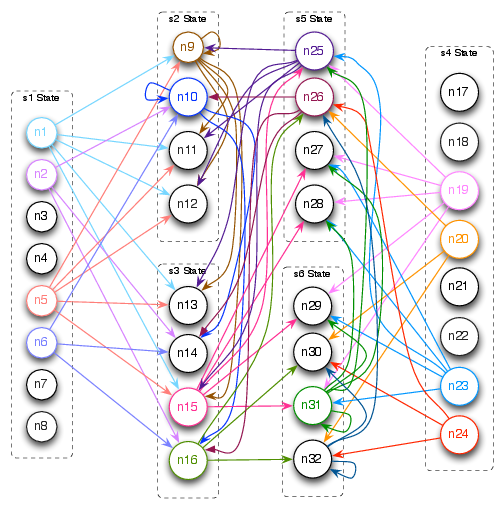
\includegraphics{example_model_checking_graph.png}
\caption{Model checking graph generated.}\end{figure}


\strong{See Also:}


{\hyperref[closure:closure.getClosure]{\code{closure.getClosure()}}}, {\hyperref[formula:formula.Formula]{\code{formula.Formula}}}, {\hyperref[modelCheckingGraph:modelCheckingGraph.getAllAtoms]{\code{getAllAtoms()}}}



\end{fulllineitems}

\index{getNoBasicFormulas() (in module modelCheckingGraph)}

\begin{fulllineitems}
\phantomsection\label{modelCheckingGraph:modelCheckingGraph.getNoBasicFormulas}\pysiglinewithargsret{\code{modelCheckingGraph.}\bfcode{getNoBasicFormulas}}{\emph{closure}}{}
Returns the formulas of the closure that are not basic formulas.
\begin{quote}\begin{description}
\item[{Parameters}] \leavevmode
\textbf{closure} (List of {\hyperref[formula:formula.Formula]{\code{Formula}}}) -- Closure of a formula.

\item[{Returns}] \leavevmode
List of formulas of the closure that are not basic formulas.

\item[{Return type}] \leavevmode
List of {\hyperref[formula:formula.Formula]{\code{Formula}}}.

\item[{Example }] \leavevmode
\end{description}\end{quote}

\begin{Verbatim}[commandchars=\\\{\}]
\PYG{g+gp}{\PYGZgt{}\PYGZgt{}\PYGZgt{} }\PYG{k+kn}{from} \PYG{n+nn}{closure} \PYG{k+kn}{import} \PYG{o}{*}
\PYG{g+gp}{\PYGZgt{}\PYGZgt{}\PYGZgt{} }\PYG{k+kn}{from} \PYG{n+nn}{modelCheckingGraph} \PYG{k+kn}{import} \PYG{o}{*}
\PYG{g+gp}{\PYGZgt{}\PYGZgt{}\PYGZgt{} }\PYG{n}{phi} \PYG{o}{=} \PYG{n}{Formula}\PYG{p}{(}\PYG{p}{\PYGZob{}}\PYG{l+s}{"}\PYG{l+s}{\PYGZlt{}\PYGZgt{}}\PYG{l+s}{"}\PYG{p}{:} \PYG{p}{\PYGZob{}}\PYG{l+s}{"}\PYG{l+s}{\PYGZca{}}\PYG{l+s}{"}\PYG{p}{:}\PYG{p}{\PYGZob{}}\PYG{l+s}{"}\PYG{l+s}{"}\PYG{p}{:}\PYG{l+s}{"}\PYG{l+s}{in=true}\PYG{l+s}{"}\PYG{p}{,}\PYG{l+s}{"}\PYG{l+s}{\PYGZti{}}\PYG{l+s}{"}\PYG{p}{:}\PYG{p}{\PYGZob{}}\PYG{l+s}{"}\PYG{l+s}{o}\PYG{l+s}{"}\PYG{p}{:}\PYG{l+s}{"}\PYG{l+s}{x=2}\PYG{l+s}{"}\PYG{p}{\PYGZcb{}}\PYG{p}{\PYGZcb{}}\PYG{p}{\PYGZcb{}}\PYG{p}{\PYGZcb{}}\PYG{p}{)}
\PYG{g+gp}{\PYGZgt{}\PYGZgt{}\PYGZgt{} }\PYG{n}{closure} \PYG{o}{=} \PYG{p}{[}\PYG{p}{]}
\PYG{g+gp}{\PYGZgt{}\PYGZgt{}\PYGZgt{} }\PYG{n}{getClosure}\PYG{p}{(}\PYG{n}{phi}\PYG{p}{,}\PYG{n}{closure}\PYG{p}{)}
\PYG{g+gp}{\PYGZgt{}\PYGZgt{}\PYGZgt{} }\PYG{n}{noBasicFormulas} \PYG{o}{=} \PYG{n}{getNoBasicFormulas}\PYG{p}{(}\PYG{n}{closure}\PYG{p}{)}
\PYG{g+gp}{\PYGZgt{}\PYGZgt{}\PYGZgt{} }\PYG{k}{for} \PYG{n}{formula} \PYG{o+ow}{in} \PYG{n}{noBasicFormulas}\PYG{p}{:}
\PYG{g+gp}{... }    \PYG{k}{print} \PYG{n}{formula}\PYG{o}{.}\PYG{n}{getFormula}\PYG{p}{(}\PYG{p}{)}
\PYG{g+gp}{... }
\PYG{g+go}{\PYGZob{}'\PYGZlt{}\PYGZgt{}': \PYGZob{}'\PYGZca{}': \PYGZob{}'': 'in=true', '\PYGZti{}': \PYGZob{}'o': 'x=2'\PYGZcb{}\PYGZcb{}\PYGZcb{}\PYGZcb{}}
\PYG{g+go}{\PYGZob{}'\PYGZca{}': \PYGZob{}'': 'in=true', '\PYGZti{}': \PYGZob{}'o': 'x=2'\PYGZcb{}\PYGZcb{}\PYGZcb{}}
\end{Verbatim}


\strong{See Also:}


{\hyperref[closure:closure.getClosure]{\code{closure.getClosure()}}}, {\hyperref[formula:formula.Formula]{\code{formula.Formula}}}



\end{fulllineitems}

\index{getTotalNodes() (in module modelCheckingGraph)}

\begin{fulllineitems}
\phantomsection\label{modelCheckingGraph:modelCheckingGraph.getTotalNodes}\pysiglinewithargsret{\code{modelCheckingGraph.}\bfcode{getTotalNodes}}{\emph{graph}}{}
Returns the total number of atoms.
\begin{quote}\begin{description}
\item[{Parameters}] \leavevmode
\textbf{graph} (\emph{Dictionary}) -- Dictionary representing the atoms in each tcc state.

\item[{Returns}] \leavevmode
The total number of atoms.

\item[{Return type}] \leavevmode
Integer

\item[{Example }] \leavevmode
\end{description}\end{quote}

\begin{Verbatim}[commandchars=\\\{\}]
\PYG{g+gp}{\PYGZgt{}\PYGZgt{}\PYGZgt{} }\PYG{k+kn}{from} \PYG{n+nn}{modelCheckingGraph} \PYG{k+kn}{import} \PYG{o}{*}
\PYG{g+go}{\PYGZgt{}\PYGZgt{}\PYGZgt{}\PYGZgt{} graph = \PYGZob{}1: [[Formula(\PYGZob{}'': 'in=true'\PYGZcb{}), Formula(\PYGZob{}'o': 'x=2'\PYGZcb{})],}
\PYG{g+gp}{... }\PYG{p}{[}\PYG{n}{Formula}\PYG{p}{(}\PYG{p}{\PYGZob{}}\PYG{l+s}{'}\PYG{l+s}{\PYGZti{}}\PYG{l+s}{'}\PYG{p}{:} \PYG{p}{\PYGZob{}}\PYG{l+s}{'}\PYG{l+s}{\PYGZca{}}\PYG{l+s}{'}\PYG{p}{:} \PYG{p}{\PYGZob{}}\PYG{l+s}{'}\PYG{l+s}{'}\PYG{p}{:} \PYG{l+s}{'}\PYG{l+s}{in=true}\PYG{l+s}{'}\PYG{p}{,} \PYG{l+s}{'}\PYG{l+s}{\PYGZti{}}\PYG{l+s}{'}\PYG{p}{:} \PYG{p}{\PYGZob{}}\PYG{l+s}{'}\PYG{l+s}{o}\PYG{l+s}{'}\PYG{p}{:} \PYG{l+s}{'}\PYG{l+s}{x=2}\PYG{l+s}{'}\PYG{p}{\PYGZcb{}}\PYG{p}{\PYGZcb{}}\PYG{p}{\PYGZcb{}}\PYG{p}{\PYGZcb{}}\PYG{p}{)}\PYG{p}{]}\PYG{p}{]}\PYG{p}{,}
\PYG{g+gp}{... }\PYG{l+m+mi}{2}\PYG{p}{:} \PYG{p}{[}\PYG{p}{[}\PYG{n}{Formula}\PYG{p}{(}\PYG{p}{\PYGZob{}}\PYG{l+s}{'}\PYG{l+s}{\PYGZti{}}\PYG{l+s}{'}\PYG{p}{:} \PYG{l+s}{'}\PYG{l+s}{in=true}\PYG{l+s}{'}\PYG{p}{\PYGZcb{}}\PYG{p}{)}\PYG{p}{,}\PYG{n}{Formula}\PYG{p}{(}\PYG{p}{\PYGZob{}}\PYG{l+s}{'}\PYG{l+s}{\PYGZti{}}\PYG{l+s}{'}\PYG{p}{:} \PYG{p}{\PYGZob{}}\PYG{l+s}{'}\PYG{l+s}{o}\PYG{l+s}{'}\PYG{p}{:} \PYG{l+s}{'}\PYG{l+s}{x=2}\PYG{l+s}{'}\PYG{p}{\PYGZcb{}}\PYG{p}{\PYGZcb{}}\PYG{p}{)}\PYG{p}{]}\PYG{p}{]}\PYG{p}{\PYGZcb{}}
\PYG{g+gp}{\PYGZgt{}\PYGZgt{}\PYGZgt{} }\PYG{n}{getTotalNodes}\PYG{p}{(}\PYG{n}{graph}\PYG{p}{)}
\PYG{g+go}{3}
\end{Verbatim}


\strong{See Also:}


{\hyperref[formula:formula.Formula]{\code{formula.Formula}}}



\end{fulllineitems}

\index{isConsistent() (in module modelCheckingGraph)}

\begin{fulllineitems}
\phantomsection\label{modelCheckingGraph:modelCheckingGraph.isConsistent}\pysiglinewithargsret{\code{modelCheckingGraph.}\bfcode{isConsistent}}{\emph{formula}, \emph{atom}}{}
Checks if a formula is consistent with the set of formulas in an atom.
\begin{quote}\begin{description}
\item[{Parameters}] \leavevmode\begin{itemize}
\item {} 
\textbf{formula} ({\hyperref[formula:formula.Formula]{\code{Formula}}}) -- Formula

\item {} 
\textbf{atom} (List of {\hyperref[formula:formula.Formula]{\code{Formula}}}.) -- List of consistent formulas representing an atom of the closure.

\end{itemize}

\item[{Returns}] \leavevmode
\code{True} if the formula is consistent with the set of formulas in the atom or \code{False} otherwise.

\item[{Return type}] \leavevmode
Boolean

\item[{Example }] \leavevmode
\end{description}\end{quote}

\begin{Verbatim}[commandchars=\\\{\}]
\PYG{g+gp}{\PYGZgt{}\PYGZgt{}\PYGZgt{} }\PYG{k+kn}{from} \PYG{n+nn}{closure} \PYG{k+kn}{import} \PYG{o}{*}
\PYG{g+gp}{\PYGZgt{}\PYGZgt{}\PYGZgt{} }\PYG{k+kn}{from} \PYG{n+nn}{modelCheckingGraph} \PYG{k+kn}{import} \PYG{o}{*}
\PYG{g+gp}{\PYGZgt{}\PYGZgt{}\PYGZgt{} }\PYG{n}{phi} \PYG{o}{=} \PYG{n}{Formula}\PYG{p}{(}\PYG{p}{\PYGZob{}}\PYG{l+s}{"}\PYG{l+s}{\PYGZlt{}\PYGZgt{}}\PYG{l+s}{"}\PYG{p}{:} \PYG{p}{\PYGZob{}}\PYG{l+s}{"}\PYG{l+s}{\PYGZca{}}\PYG{l+s}{"}\PYG{p}{:}\PYG{p}{\PYGZob{}}\PYG{l+s}{"}\PYG{l+s}{"}\PYG{p}{:}\PYG{l+s}{"}\PYG{l+s}{in=true}\PYG{l+s}{"}\PYG{p}{,}\PYG{l+s}{"}\PYG{l+s}{\PYGZti{}}\PYG{l+s}{"}\PYG{p}{:}\PYG{p}{\PYGZob{}}\PYG{l+s}{"}\PYG{l+s}{o}\PYG{l+s}{"}\PYG{p}{:}\PYG{l+s}{"}\PYG{l+s}{x=2}\PYG{l+s}{"}\PYG{p}{\PYGZcb{}}\PYG{p}{\PYGZcb{}}\PYG{p}{\PYGZcb{}}\PYG{p}{\PYGZcb{}}\PYG{p}{)}
\PYG{g+gp}{\PYGZgt{}\PYGZgt{}\PYGZgt{} }\PYG{n}{closure} \PYG{o}{=} \PYG{p}{[}\PYG{p}{]}
\PYG{g+gp}{\PYGZgt{}\PYGZgt{}\PYGZgt{} }\PYG{n}{getClosure}\PYG{p}{(}\PYG{n}{phi}\PYG{p}{,}\PYG{n}{closure}\PYG{p}{)}
\PYG{g+gp}{\PYGZgt{}\PYGZgt{}\PYGZgt{} }\PYG{n}{atoms} \PYG{o}{=} \PYG{n}{getAllAtoms}\PYG{p}{(}\PYG{n}{closure}\PYG{p}{)}
\PYG{g+gp}{\PYGZgt{}\PYGZgt{}\PYGZgt{} }\PYG{n}{isConsistent}\PYG{p}{(}\PYG{n}{Formula}\PYG{p}{(}\PYG{p}{\PYGZob{}}\PYG{l+s}{'}\PYG{l+s}{'}\PYG{p}{:} \PYG{l+s}{'}\PYG{l+s}{x=1}\PYG{l+s}{'}\PYG{p}{\PYGZcb{}}\PYG{p}{)}\PYG{p}{,} \PYG{n}{atoms}\PYG{p}{[}\PYG{l+m+mi}{0}\PYG{p}{]}\PYG{p}{)}
\PYG{g+go}{False}
\end{Verbatim}


\strong{See Also:}


{\hyperref[closure:closure.getClosure]{\code{closure.getClosure()}}}, {\hyperref[formula:formula.Formula]{\code{formula.Formula}}}, {\hyperref[modelCheckingGraph:modelCheckingGraph.getAllAtoms]{\code{getAllAtoms()}}}



\begin{notice}{note}{Note:}
This function is based on the conditions shown in the defintion 6.1 of the thesis document.
\end{notice}

\end{fulllineitems}

\index{isInAtom() (in module modelCheckingGraph)}

\begin{fulllineitems}
\phantomsection\label{modelCheckingGraph:modelCheckingGraph.isInAtom}\pysiglinewithargsret{\code{modelCheckingGraph.}\bfcode{isInAtom}}{\emph{formula}, \emph{atom}}{}
Checks if a formula is in an atom.
\begin{quote}\begin{description}
\item[{Parameters}] \leavevmode\begin{itemize}
\item {} 
\textbf{formula} (\emph{Dictionary}) -- Structure representing a formula.

\item {} 
\textbf{atom} (List of {\hyperref[formula:formula.Formula]{\code{Formula}}}.) -- List of consistent formulas representing an atom of the closure.

\end{itemize}

\item[{Returns}] \leavevmode
\code{True} if the formula is in atom or \code{False} otherwise.

\item[{Return type}] \leavevmode
Boolean

\item[{Example }] \leavevmode
\end{description}\end{quote}

\begin{Verbatim}[commandchars=\\\{\}]
\PYG{g+gp}{\PYGZgt{}\PYGZgt{}\PYGZgt{} }\PYG{k+kn}{from} \PYG{n+nn}{closure} \PYG{k+kn}{import} \PYG{o}{*}
\PYG{g+gp}{\PYGZgt{}\PYGZgt{}\PYGZgt{} }\PYG{k+kn}{from} \PYG{n+nn}{modelCheckingGraph} \PYG{k+kn}{import} \PYG{o}{*}
\PYG{g+gp}{\PYGZgt{}\PYGZgt{}\PYGZgt{} }\PYG{n}{phi} \PYG{o}{=} \PYG{n}{Formula}\PYG{p}{(}\PYG{p}{\PYGZob{}}\PYG{l+s}{"}\PYG{l+s}{\PYGZlt{}\PYGZgt{}}\PYG{l+s}{"}\PYG{p}{:} \PYG{p}{\PYGZob{}}\PYG{l+s}{"}\PYG{l+s}{\PYGZca{}}\PYG{l+s}{"}\PYG{p}{:}\PYG{p}{\PYGZob{}}\PYG{l+s}{"}\PYG{l+s}{"}\PYG{p}{:}\PYG{l+s}{"}\PYG{l+s}{in=true}\PYG{l+s}{"}\PYG{p}{,}\PYG{l+s}{"}\PYG{l+s}{\PYGZti{}}\PYG{l+s}{"}\PYG{p}{:}\PYG{p}{\PYGZob{}}\PYG{l+s}{"}\PYG{l+s}{o}\PYG{l+s}{"}\PYG{p}{:}\PYG{l+s}{"}\PYG{l+s}{x=2}\PYG{l+s}{"}\PYG{p}{\PYGZcb{}}\PYG{p}{\PYGZcb{}}\PYG{p}{\PYGZcb{}}\PYG{p}{\PYGZcb{}}\PYG{p}{)}
\PYG{g+gp}{\PYGZgt{}\PYGZgt{}\PYGZgt{} }\PYG{n}{closure} \PYG{o}{=} \PYG{p}{[}\PYG{p}{]}
\PYG{g+gp}{\PYGZgt{}\PYGZgt{}\PYGZgt{} }\PYG{n}{getClosure}\PYG{p}{(}\PYG{n}{phi}\PYG{p}{,}\PYG{n}{closure}\PYG{p}{)}
\PYG{g+gp}{\PYGZgt{}\PYGZgt{}\PYGZgt{} }\PYG{n}{atoms} \PYG{o}{=} \PYG{n}{getAllAtoms}\PYG{p}{(}\PYG{n}{closure}\PYG{p}{)}
\PYG{g+gp}{\PYGZgt{}\PYGZgt{}\PYGZgt{} }\PYG{n}{isInAtom}\PYG{p}{(}\PYG{p}{\PYGZob{}}\PYG{l+s}{'}\PYG{l+s}{'}\PYG{p}{:} \PYG{l+s}{'}\PYG{l+s}{in=true}\PYG{l+s}{'}\PYG{p}{\PYGZcb{}}\PYG{p}{,} \PYG{n}{atoms}\PYG{p}{[}\PYG{l+m+mi}{0}\PYG{p}{]}\PYG{p}{)}
\PYG{g+go}{True}
\end{Verbatim}


\strong{See Also:}


{\hyperref[closure:closure.getClosure]{\code{closure.getClosure()}}}, {\hyperref[formula:formula.Formula]{\code{formula.Formula}}}, {\hyperref[modelCheckingGraph:modelCheckingGraph.getAllAtoms]{\code{getAllAtoms()}}}



\end{fulllineitems}

\index{isNextState() (in module modelCheckingGraph)}

\begin{fulllineitems}
\phantomsection\label{modelCheckingGraph:modelCheckingGraph.isNextState}\pysiglinewithargsret{\code{modelCheckingGraph.}\bfcode{isNextState}}{\emph{nextFormulas}, \emph{nextAtom}}{}
Checks if an atom satisfies a list of formulas with next operator as main connective.
\begin{quote}\begin{description}
\item[{Parameters}] \leavevmode\begin{itemize}
\item {} 
\textbf{nextFormulas} (List of {\hyperref[formula:formula.Formula]{\code{Formula}}}) -- List of formulas with next operator as main connective.

\item {} 
\textbf{nextAtom} (List of {\hyperref[formula:formula.Formula]{\code{Formula}}}) -- Atom.

\end{itemize}

\item[{Returns}] \leavevmode
\code{True} if the atom satisfies the termporal formulas or \code{False} otherwise.

\item[{Return type}] \leavevmode
Boolean

\item[{Example }] \leavevmode
\end{description}\end{quote}

\begin{Verbatim}[commandchars=\\\{\}]
\PYG{g+gp}{\PYGZgt{}\PYGZgt{}\PYGZgt{} }\PYG{k+kn}{from} \PYG{n+nn}{modelCheckingGraph} \PYG{k+kn}{import} \PYG{o}{*}
\PYG{g+gp}{\PYGZgt{}\PYGZgt{}\PYGZgt{} }\PYG{n}{atom} \PYG{o}{=} \PYG{p}{[}\PYG{n}{Formula}\PYG{p}{(}\PYG{p}{\PYGZob{}}\PYG{l+s}{'}\PYG{l+s}{o}\PYG{l+s}{'}\PYG{p}{:} \PYG{p}{\PYGZob{}}\PYG{l+s}{'}\PYG{l+s}{\PYGZlt{}\PYGZgt{}}\PYG{l+s}{'}\PYG{p}{:} \PYG{p}{\PYGZob{}}\PYG{l+s}{'}\PYG{l+s}{\PYGZca{}}\PYG{l+s}{'}\PYG{p}{:} \PYG{p}{\PYGZob{}}\PYG{l+s}{'}\PYG{l+s}{'}\PYG{p}{:} \PYG{l+s}{'}\PYG{l+s}{in=true}\PYG{l+s}{'}\PYG{p}{,} \PYG{l+s}{'}\PYG{l+s}{\PYGZti{}}\PYG{l+s}{'}\PYG{p}{:} \PYG{p}{\PYGZob{}}\PYG{l+s}{'}\PYG{l+s}{o}\PYG{l+s}{'}\PYG{p}{:} \PYG{l+s}{'}\PYG{l+s}{x=2}\PYG{l+s}{'}\PYG{p}{\PYGZcb{}}\PYG{p}{\PYGZcb{}}\PYG{p}{\PYGZcb{}}\PYG{p}{\PYGZcb{}}\PYG{p}{\PYGZcb{}}\PYG{p}{)}\PYG{p}{,}
\PYG{g+gp}{... }\PYG{n}{Formula}\PYG{p}{(}\PYG{p}{\PYGZob{}}\PYG{l+s}{'}\PYG{l+s}{'}\PYG{p}{:} \PYG{l+s}{'}\PYG{l+s}{in=true}\PYG{l+s}{'}\PYG{p}{\PYGZcb{}}\PYG{p}{)}\PYG{p}{,} \PYG{n}{Formula}\PYG{p}{(}\PYG{p}{\PYGZob{}}\PYG{l+s}{'}\PYG{l+s}{o}\PYG{l+s}{'}\PYG{p}{:} \PYG{l+s}{'}\PYG{l+s}{x=2}\PYG{l+s}{'}\PYG{p}{\PYGZcb{}}\PYG{p}{)}\PYG{p}{,} \PYG{n}{Formula}\PYG{p}{(}\PYG{p}{\PYGZob{}}\PYG{l+s}{'}\PYG{l+s}{'}\PYG{p}{:} \PYG{l+s}{'}\PYG{l+s}{x=2}\PYG{l+s}{'}\PYG{p}{\PYGZcb{}}\PYG{p}{)}\PYG{p}{,}
\PYG{g+gp}{... }\PYG{n}{Formula}\PYG{p}{(}\PYG{p}{\PYGZob{}}\PYG{l+s}{'}\PYG{l+s}{\PYGZlt{}\PYGZgt{}}\PYG{l+s}{'}\PYG{p}{:} \PYG{p}{\PYGZob{}}\PYG{l+s}{'}\PYG{l+s}{\PYGZca{}}\PYG{l+s}{'}\PYG{p}{:} \PYG{p}{\PYGZob{}}\PYG{l+s}{'}\PYG{l+s}{'}\PYG{p}{:} \PYG{l+s}{'}\PYG{l+s}{in=true}\PYG{l+s}{'}\PYG{p}{,} \PYG{l+s}{'}\PYG{l+s}{\PYGZti{}}\PYG{l+s}{'}\PYG{p}{:} \PYG{p}{\PYGZob{}}\PYG{l+s}{'}\PYG{l+s}{o}\PYG{l+s}{'}\PYG{p}{:} \PYG{l+s}{'}\PYG{l+s}{x=2}\PYG{l+s}{'}\PYG{p}{\PYGZcb{}}\PYG{p}{\PYGZcb{}}\PYG{p}{\PYGZcb{}}\PYG{p}{\PYGZcb{}}\PYG{p}{)}\PYG{p}{,}
\PYG{g+gp}{... }\PYG{n}{Formula}\PYG{p}{(}\PYG{p}{\PYGZob{}}\PYG{l+s}{'}\PYG{l+s}{\PYGZti{}}\PYG{l+s}{'}\PYG{p}{:} \PYG{p}{\PYGZob{}}\PYG{l+s}{'}\PYG{l+s}{\PYGZca{}}\PYG{l+s}{'}\PYG{p}{:} \PYG{p}{\PYGZob{}}\PYG{l+s}{'}\PYG{l+s}{'}\PYG{p}{:} \PYG{l+s}{'}\PYG{l+s}{in=true}\PYG{l+s}{'}\PYG{p}{,} \PYG{l+s}{'}\PYG{l+s}{\PYGZti{}}\PYG{l+s}{'}\PYG{p}{:} \PYG{p}{\PYGZob{}}\PYG{l+s}{'}\PYG{l+s}{o}\PYG{l+s}{'}\PYG{p}{:} \PYG{l+s}{'}\PYG{l+s}{x=2}\PYG{l+s}{'}\PYG{p}{\PYGZcb{}}\PYG{p}{\PYGZcb{}}\PYG{p}{\PYGZcb{}}\PYG{p}{\PYGZcb{}}\PYG{p}{)}\PYG{p}{]}
\PYG{g+gp}{\PYGZgt{}\PYGZgt{}\PYGZgt{} }
\PYG{g+gp}{\PYGZgt{}\PYGZgt{}\PYGZgt{} }\PYG{n}{formulas} \PYG{o}{=} \PYG{p}{[}\PYG{n}{Formula}\PYG{p}{(}\PYG{p}{\PYGZob{}}\PYG{l+s}{'}\PYG{l+s}{o}\PYG{l+s}{'}\PYG{p}{:} \PYG{l+s}{'}\PYG{l+s}{x=2}\PYG{l+s}{'}\PYG{p}{\PYGZcb{}}\PYG{p}{)}\PYG{p}{]}
\PYG{g+gp}{\PYGZgt{}\PYGZgt{}\PYGZgt{} }\PYG{n}{isNextState}\PYG{p}{(}\PYG{n}{formulas}\PYG{p}{,}\PYG{n}{atom}\PYG{p}{)}
\PYG{g+go}{True}
\end{Verbatim}

\begin{notice}{note}{Note:}
We say that an atom satisfies a list of formulas when for all the formulas $\circ\phi$ in the list we found a formula $\phi$ in the atom.
\end{notice}


\strong{See Also:}


{\hyperref[formula:formula.Formula]{\code{formula.Formula}}}



\end{fulllineitems}

\index{list2dict() (in module modelCheckingGraph)}

\begin{fulllineitems}
\phantomsection\label{modelCheckingGraph:modelCheckingGraph.list2dict}\pysiglinewithargsret{\code{modelCheckingGraph.}\bfcode{list2dict}}{\emph{lists}, \emph{offset}}{}
Converts a list to a dictionary with ascending numbers as keys.
\begin{quote}\begin{description}
\item[{Parameters}] \leavevmode\begin{itemize}
\item {} 
\textbf{lists} (\emph{List}) -- List with elements.

\item {} 
\textbf{offset} (\emph{Integer}) -- Offset of numeration.

\end{itemize}

\item[{Returns}] \leavevmode
Dictionary with numbers as keys, and elements of the list as values.

\item[{Return type}] \leavevmode
Dictionary.

\item[{Example }] \leavevmode
\end{description}\end{quote}

\begin{Verbatim}[commandchars=\\\{\}]
\PYG{g+gp}{\PYGZgt{}\PYGZgt{}\PYGZgt{} }\PYG{k+kn}{from} \PYG{n+nn}{modelCheckingGraph} \PYG{k+kn}{import} \PYG{o}{*}
\PYG{g+gp}{\PYGZgt{}\PYGZgt{}\PYGZgt{} }\PYG{n+nb}{list} \PYG{o}{=} \PYG{p}{[}\PYG{l+s}{"}\PYG{l+s}{I}\PYG{l+s}{"}\PYG{p}{,} \PYG{l+s}{"}\PYG{l+s}{Love}\PYG{l+s}{"}\PYG{p}{,} \PYG{l+s}{"}\PYG{l+s}{Computer}\PYG{l+s}{"}\PYG{p}{,} \PYG{l+s}{"}\PYG{l+s}{Science}\PYG{l+s}{"}\PYG{p}{]}
\PYG{g+gp}{\PYGZgt{}\PYGZgt{}\PYGZgt{} }\PYG{n}{list2dict}\PYG{p}{(}\PYG{n+nb}{list}\PYG{p}{,} \PYG{l+m+mi}{2}\PYG{p}{)}
\PYG{g+go}{\PYGZob{}2: 'I', 3: 'Love', 4: 'Computer', 5: 'Science'\PYGZcb{}}
\end{Verbatim}

\end{fulllineitems}

\index{propositionConsistent() (in module modelCheckingGraph)}

\begin{fulllineitems}
\phantomsection\label{modelCheckingGraph:modelCheckingGraph.propositionConsistent}\pysiglinewithargsret{\code{modelCheckingGraph.}\bfcode{propositionConsistent}}{\emph{formula}, \emph{atom}}{}
Checks if a proposition is consistent with the formulas of an atom.
\begin{quote}\begin{description}
\item[{Parameters}] \leavevmode\begin{itemize}
\item {} 
\textbf{formula} ({\hyperref[formula:formula.Formula]{\code{Formula}}}) -- Formula

\item {} 
\textbf{atom} (List of {\hyperref[formula:formula.Formula]{\code{Formula}}}) -- Atom

\end{itemize}

\item[{Returns}] \leavevmode
\code{True} if the proposition is consistent with the atom or \code{False} otherwise.

\item[{Return type}] \leavevmode
Boolean.

\item[{Example }] \leavevmode
\end{description}\end{quote}

\begin{Verbatim}[commandchars=\\\{\}]
\PYG{g+gp}{\PYGZgt{}\PYGZgt{}\PYGZgt{} }\PYG{k+kn}{from} \PYG{n+nn}{closure} \PYG{k+kn}{import} \PYG{o}{*}
\PYG{g+gp}{\PYGZgt{}\PYGZgt{}\PYGZgt{} }\PYG{k+kn}{from} \PYG{n+nn}{modelCheckingGraph} \PYG{k+kn}{import} \PYG{o}{*}
\PYG{g+gp}{\PYGZgt{}\PYGZgt{}\PYGZgt{} }\PYG{n}{phi} \PYG{o}{=} \PYG{n}{Formula}\PYG{p}{(}\PYG{p}{\PYGZob{}}\PYG{l+s}{"}\PYG{l+s}{\PYGZlt{}\PYGZgt{}}\PYG{l+s}{"}\PYG{p}{:} \PYG{p}{\PYGZob{}}\PYG{l+s}{"}\PYG{l+s}{\PYGZca{}}\PYG{l+s}{"}\PYG{p}{:}\PYG{p}{\PYGZob{}}\PYG{l+s}{"}\PYG{l+s}{"}\PYG{p}{:}\PYG{l+s}{"}\PYG{l+s}{in=true}\PYG{l+s}{"}\PYG{p}{,}\PYG{l+s}{"}\PYG{l+s}{\PYGZti{}}\PYG{l+s}{"}\PYG{p}{:}\PYG{p}{\PYGZob{}}\PYG{l+s}{"}\PYG{l+s}{o}\PYG{l+s}{"}\PYG{p}{:}\PYG{l+s}{"}\PYG{l+s}{x=2}\PYG{l+s}{"}\PYG{p}{\PYGZcb{}}\PYG{p}{\PYGZcb{}}\PYG{p}{\PYGZcb{}}\PYG{p}{\PYGZcb{}}\PYG{p}{)}
\PYG{g+gp}{\PYGZgt{}\PYGZgt{}\PYGZgt{} }\PYG{n}{closure} \PYG{o}{=} \PYG{p}{[}\PYG{p}{]}
\PYG{g+gp}{\PYGZgt{}\PYGZgt{}\PYGZgt{} }\PYG{n}{getClosure}\PYG{p}{(}\PYG{n}{phi}\PYG{p}{,}\PYG{n}{closure}\PYG{p}{)}
\PYG{g+gp}{\PYGZgt{}\PYGZgt{}\PYGZgt{} }\PYG{n}{atoms} \PYG{o}{=} \PYG{n}{getAllAtoms}\PYG{p}{(}\PYG{n}{closure}\PYG{p}{)}
\PYG{g+gp}{\PYGZgt{}\PYGZgt{}\PYGZgt{} }\PYG{n}{proposition} \PYG{o}{=} \PYG{n}{Formula}\PYG{p}{(}\PYG{p}{\PYGZob{}}\PYG{l+s}{"}\PYG{l+s}{\PYGZti{}}\PYG{l+s}{"}\PYG{p}{:}\PYG{l+s}{"}\PYG{l+s}{x=2}\PYG{l+s}{"}\PYG{p}{\PYGZcb{}}\PYG{p}{)}
\PYG{g+gp}{\PYGZgt{}\PYGZgt{}\PYGZgt{} }\PYG{n}{atom} \PYG{o}{=} \PYG{n}{atoms}\PYG{p}{[}\PYG{l+m+mi}{0}\PYG{p}{]}
\PYG{g+gp}{\PYGZgt{}\PYGZgt{}\PYGZgt{} }\PYG{k}{for} \PYG{n}{formula} \PYG{o+ow}{in} \PYG{n}{atom}\PYG{p}{:}
\PYG{g+gp}{... }    \PYG{k}{print} \PYG{n}{formula}\PYG{o}{.}\PYG{n}{getFormula}\PYG{p}{(}\PYG{p}{)}
\PYG{g+gp}{... }
\PYG{g+go}{\PYGZob{}'o': \PYGZob{}'\PYGZlt{}\PYGZgt{}': \PYGZob{}'\PYGZca{}': \PYGZob{}'': 'in=true', '\PYGZti{}': \PYGZob{}'o': 'x=2'\PYGZcb{}\PYGZcb{}\PYGZcb{}\PYGZcb{}\PYGZcb{}}
\PYG{g+go}{\PYGZob{}'': 'in=true'\PYGZcb{}}
\PYG{g+go}{\PYGZob{}'o': 'x=2'\PYGZcb{}}
\PYG{g+go}{\PYGZob{}'': 'x=2'\PYGZcb{}}
\PYG{g+go}{\PYGZob{}'\PYGZlt{}\PYGZgt{}': \PYGZob{}'\PYGZca{}': \PYGZob{}'': 'in=true', '\PYGZti{}': \PYGZob{}'o': 'x=2'\PYGZcb{}\PYGZcb{}\PYGZcb{}\PYGZcb{}}
\PYG{g+go}{\PYGZob{}'\PYGZti{}': \PYGZob{}'\PYGZca{}': \PYGZob{}'': 'in=true', '\PYGZti{}': \PYGZob{}'o': 'x=2'\PYGZcb{}\PYGZcb{}\PYGZcb{}\PYGZcb{}}
\PYG{g+gp}{\PYGZgt{}\PYGZgt{}\PYGZgt{} }\PYG{n}{propositionConsistent}\PYG{p}{(}\PYG{n}{proposition}\PYG{p}{,} \PYG{n}{atom}\PYG{p}{)}
\PYG{g+go}{False}
\end{Verbatim}


\strong{See Also:}


{\hyperref[closure:closure.getClosure]{\code{closure.getClosure()}}}, {\hyperref[formula:formula.Formula]{\code{formula.Formula}}}, {\hyperref[modelCheckingGraph:modelCheckingGraph.getAllAtoms]{\code{getAllAtoms()}}}



\end{fulllineitems}

\index{searchFormulas() (in module modelCheckingGraph)}

\begin{fulllineitems}
\phantomsection\label{modelCheckingGraph:modelCheckingGraph.searchFormulas}\pysiglinewithargsret{\code{modelCheckingGraph.}\bfcode{searchFormulas}}{\emph{formulas}, \emph{connective}}{}
Returns the formulas that have a particular main connective.
\begin{quote}\begin{description}
\item[{Parameters}] \leavevmode\begin{itemize}
\item {} 
\textbf{formulas} (List of {\hyperref[formula:formula.Formula]{\code{Formula}}}) -- List of formulas.

\item {} 
\textbf{connective} (\emph{String}) -- The main connective.

\end{itemize}

\item[{Returns}] \leavevmode
List containing the formulas that have the main connective.

\item[{Return type}] \leavevmode
List

\item[{Example }] \leavevmode
\end{description}\end{quote}

\begin{Verbatim}[commandchars=\\\{\}]
\PYG{g+gp}{\PYGZgt{}\PYGZgt{}\PYGZgt{} }\PYG{k+kn}{from} \PYG{n+nn}{modelCheckingGraph} \PYG{k+kn}{import} \PYG{o}{*}
\PYG{g+gp}{\PYGZgt{}\PYGZgt{}\PYGZgt{} }\PYG{n+nb}{list} \PYG{o}{=} \PYG{p}{[}\PYG{n}{Formula}\PYG{p}{(}\PYG{p}{\PYGZob{}}\PYG{l+s}{'}\PYG{l+s}{o}\PYG{l+s}{'}\PYG{p}{:} \PYG{l+s}{'}\PYG{l+s}{x=2}\PYG{l+s}{'}\PYG{p}{\PYGZcb{}}\PYG{p}{)}\PYG{p}{,} \PYG{n}{Formula}\PYG{p}{(}\PYG{p}{\PYGZob{}}\PYG{l+s}{'}\PYG{l+s}{\PYGZti{}}\PYG{l+s}{'}\PYG{p}{:} \PYG{p}{\PYGZob{}}\PYG{l+s}{'}\PYG{l+s}{o}\PYG{l+s}{'}\PYG{p}{:} \PYG{l+s}{'}\PYG{l+s}{x=2}\PYG{l+s}{'}\PYG{p}{\PYGZcb{}}\PYG{p}{\PYGZcb{}}\PYG{p}{)}\PYG{p}{,} \PYG{n}{Formula}\PYG{p}{(}\PYG{p}{\PYGZob{}}\PYG{l+s}{'}\PYG{l+s}{o}\PYG{l+s}{'}\PYG{p}{:} \PYG{p}{\PYGZob{}}\PYG{l+s}{'}\PYG{l+s}{\PYGZti{}}\PYG{l+s}{'}\PYG{p}{:} \PYG{l+s}{'}\PYG{l+s}{x=2}\PYG{l+s}{'}\PYG{p}{\PYGZcb{}}\PYG{p}{\PYGZcb{}}\PYG{p}{)}\PYG{p}{]}
\PYG{g+gp}{\PYGZgt{}\PYGZgt{}\PYGZgt{} }\PYG{n}{result} \PYG{o}{=} \PYG{n}{searchFormulas}\PYG{p}{(}\PYG{n+nb}{list}\PYG{p}{,}\PYG{l+s}{'}\PYG{l+s}{o}\PYG{l+s}{'}\PYG{p}{)}
\PYG{g+gp}{\PYGZgt{}\PYGZgt{}\PYGZgt{} }\PYG{k}{for} \PYG{n}{formula} \PYG{o+ow}{in} \PYG{n}{result}\PYG{p}{:}
\PYG{g+gp}{... }    \PYG{k}{print} \PYG{n}{formula}\PYG{o}{.}\PYG{n}{getFormula}\PYG{p}{(}\PYG{p}{)}
\PYG{g+gp}{... }
\PYG{g+go}{\PYGZob{}'o': 'x=2'\PYGZcb{}}
\PYG{g+go}{\PYGZob{}'o': \PYGZob{}'\PYGZti{}': 'x=2'\PYGZcb{}\PYGZcb{}}
\end{Verbatim}

\end{fulllineitems}



\chapter{Searching Algorithm}
\label{searchingAlgorithm:searching-algorithm}\label{searchingAlgorithm:module-searchingAlgorithm}\label{searchingAlgorithm::doc}\index{searchingAlgorithm (module)}
This module contains the necessary functions to check if a model checking graph satisfies a property.
\index{getFormulas() (in module searchingAlgorithm)}

\begin{fulllineitems}
\phantomsection\label{searchingAlgorithm:searchingAlgorithm.getFormulas}\pysiglinewithargsret{\code{searchingAlgorithm.}\bfcode{getFormulas}}{\emph{node}, \emph{model\_checking\_atoms}}{}
Returns the formulas of a specific model checking node.
\begin{quote}\begin{description}
\item[{Parameters}] \leavevmode\begin{itemize}
\item {} 
\textbf{node} (\emph{Integer}) -- Number of the model checking node.

\item {} 
\textbf{model\_checking\_atoms} (\emph{List of atoms.}) -- Model checking atoms.

\end{itemize}

\item[{Returns}] \leavevmode
List of formulas of the node.

\item[{Return type}] \leavevmode
List of {\hyperref[formula:formula.Formula]{\code{Formula}}}.

\item[{Example }] \leavevmode
\end{description}\end{quote}

\begin{Verbatim}[commandchars=\\\{\}]
\PYG{g+gp}{\PYGZgt{}\PYGZgt{}\PYGZgt{} }\PYG{k+kn}{from} \PYG{n+nn}{searchingAlgorithm} \PYG{k+kn}{import} \PYG{o}{*}
\PYG{g+gp}{\PYGZgt{}\PYGZgt{}\PYGZgt{} }\PYG{n}{formulas} \PYG{o}{=} \PYG{n}{getFormulas}\PYG{p}{(}\PYG{l+m+mi}{3}\PYG{p}{,} \PYG{n}{model\PYGZus{}checking\PYGZus{}atoms}\PYG{p}{)}
\PYG{g+gp}{\PYGZgt{}\PYGZgt{}\PYGZgt{} }\PYG{k}{for} \PYG{n}{formula} \PYG{o+ow}{in} \PYG{n}{basicFormulas}\PYG{p}{:}
\PYG{g+gp}{... }    \PYG{k}{print} \PYG{n}{formula}\PYG{o}{.}\PYG{n}{getFormula}\PYG{p}{(}\PYG{p}{)}
\PYG{g+go}{\PYGZob{}'o': \PYGZob{}'\PYGZlt{}\PYGZgt{}': \PYGZob{}'\PYGZca{}': \PYGZob{}'': 'in=true', '\PYGZti{}': \PYGZob{}'o': 'x=1'\PYGZcb{}\PYGZcb{}\PYGZcb{}\PYGZcb{}\PYGZcb{}}
\PYG{g+go}{\PYGZob{}'': 'in=true'\PYGZcb{}}
\PYG{g+go}{\PYGZob{}'\PYGZti{}': \PYGZob{}'o': 'x=1'\PYGZcb{}\PYGZcb{}}
\PYG{g+go}{\PYGZob{}'': 'x=1'\PYGZcb{}}
\PYG{g+go}{\PYGZob{}'o': \PYGZob{}'\PYGZti{}': 'x=1'\PYGZcb{}\PYGZcb{}}
\PYG{g+go}{\PYGZob{}'\PYGZlt{}\PYGZgt{}': \PYGZob{}'\PYGZca{}': \PYGZob{}'': 'in=true', '\PYGZti{}': \PYGZob{}'o': 'x=1'\PYGZcb{}\PYGZcb{}\PYGZcb{}\PYGZcb{}}
\PYG{g+go}{\PYGZob{}'\PYGZca{}': \PYGZob{}'': 'in=true', '\PYGZti{}': \PYGZob{}'o': 'x=1'\PYGZcb{}\PYGZcb{}\PYGZcb{}}
\end{Verbatim}


\strong{See Also:}


{\hyperref[modelCheckingGraph:modelCheckingGraph.getModelCheckingAtoms]{\code{modelCheckingGraph.getModelCheckingAtoms()}}}



\end{fulllineitems}

\index{getInitialNodes() (in module searchingAlgorithm)}

\begin{fulllineitems}
\phantomsection\label{searchingAlgorithm:searchingAlgorithm.getInitialNodes}\pysiglinewithargsret{\code{searchingAlgorithm.}\bfcode{getInitialNodes}}{\emph{tcc\_structure}, \emph{model\_checking\_atoms}}{}
Returns the initial nodes of a model checking graph.
\begin{quote}\begin{description}
\item[{Parameters}] \leavevmode\begin{itemize}
\item {} 
\textbf{tcc\_structure} (\emph{Dictionary}) -- tcc structure.

\item {} 
\textbf{model\_checking\_atoms} (\emph{Dictionary.}) -- Model checking atoms.

\end{itemize}

\item[{Returns}] \leavevmode
A list with the number of the nodes that are initial nodes.

\item[{Return type}] \leavevmode
List of Integers

\item[{Example }] \leavevmode
\end{description}\end{quote}

\begin{Verbatim}[commandchars=\\\{\}]
\PYG{g+gp}{\PYGZgt{}\PYGZgt{}\PYGZgt{} }\PYG{k+kn}{from} \PYG{n+nn}{searchingAlgorithm} \PYG{k+kn}{import} \PYG{o}{*}
\PYG{g+gp}{\PYGZgt{}\PYGZgt{}\PYGZgt{} }\PYG{n}{getInitialNodes}\PYG{p}{(}\PYG{n}{tcc\PYGZus{}structure}\PYG{p}{,}\PYG{n}{model\PYGZus{}checking\PYGZus{}atoms}\PYG{p}{)}
\PYG{g+go}{[1, 2, 3, 4, 5, 6, 7, 8, 17, 18, 19, 20, 21, 22, 23, 24]}
\end{Verbatim}


\strong{See Also:}


{\hyperref[modelCheckingGraph:modelCheckingGraph.getModelCheckingAtoms]{\code{modelCheckingGraph.getModelCheckingAtoms()}}}



\end{fulllineitems}

\index{getModelCheckingSCCSubgraphs() (in module searchingAlgorithm)}

\begin{fulllineitems}
\phantomsection\label{searchingAlgorithm:searchingAlgorithm.getModelCheckingSCCSubgraphs}\pysiglinewithargsret{\code{searchingAlgorithm.}\bfcode{getModelCheckingSCCSubgraphs}}{\emph{scc\_list}, \emph{tcc\_structure}, \emph{model\_checking\_atoms}, \emph{model\_checking\_graph}}{}
Returns the Strongly Connected Component (SCC) subgraphs of a model checking graph.
\begin{quote}\begin{description}
\item[{Parameters}] \leavevmode\begin{itemize}
\item {} 
\textbf{scc\_list} (\emph{List of Lists}) -- List of the nodes corresponding to all of SCCs in the model checking graph.

\item {} 
\textbf{tcc\_structure} (\emph{Dictionary}) -- tcc structure that represents the behavior of the system.

\item {} 
\textbf{model\_checking\_atoms} (\emph{List of atoms}) -- Model checking atoms.

\item {} 
\textbf{model\_checking\_graph} (\emph{Dictionary}) -- Model Checking graph

\end{itemize}

\item[{Returns}] \leavevmode
A list with the SCC subgraphs.

\item[{Return type}] \leavevmode
List

\item[{Example }] \leavevmode
\end{description}\end{quote}

\begin{Verbatim}[commandchars=\\\{\}]
\PYG{g+gp}{\PYGZgt{}\PYGZgt{}\PYGZgt{} }\PYG{k+kn}{from} \PYG{n+nn}{searchingAlgorithm} \PYG{k+kn}{import} \PYG{o}{*}
\PYG{g+gp}{\PYGZgt{}\PYGZgt{}\PYGZgt{} }\PYG{k+kn}{from} \PYG{n+nn}{tarjan} \PYG{k+kn}{import} \PYG{n}{tarjan}
\PYG{g+gp}{\PYGZgt{}\PYGZgt{}\PYGZgt{} }\PYG{n}{strongly\PYGZus{}connected\PYGZus{}components} \PYG{o}{=} \PYG{n}{tarjan}\PYG{p}{(}\PYG{n}{model\PYGZus{}checking\PYGZus{}graph}\PYG{p}{)}
\PYG{g+gp}{\PYGZgt{}\PYGZgt{}\PYGZgt{} }\PYG{n}{getModelCheckingSCCSubgraphs}\PYG{p}{(}\PYG{n}{strongly\PYGZus{}connected\PYGZus{}components}\PYG{p}{,} \PYG{n}{tcc\PYGZus{}structure}\PYG{p}{,} \PYG{n}{model\PYGZus{}checking\PYGZus{}atoms}\PYG{p}{,}\PYG{n}{model\PYGZus{}checking\PYGZus{}graph}\PYG{p}{)}
\PYG{g+go}{[\PYGZob{}3: [11, 13], 7: [11, 13], 11: [11, 13], 13: [27, 29], 17: [27, 29], 21: [27, 29], 27: [11, 13], 29: [27, 29]\PYGZcb{}]}
\end{Verbatim}
\begin{figure}[htbp]
\centering
\capstart

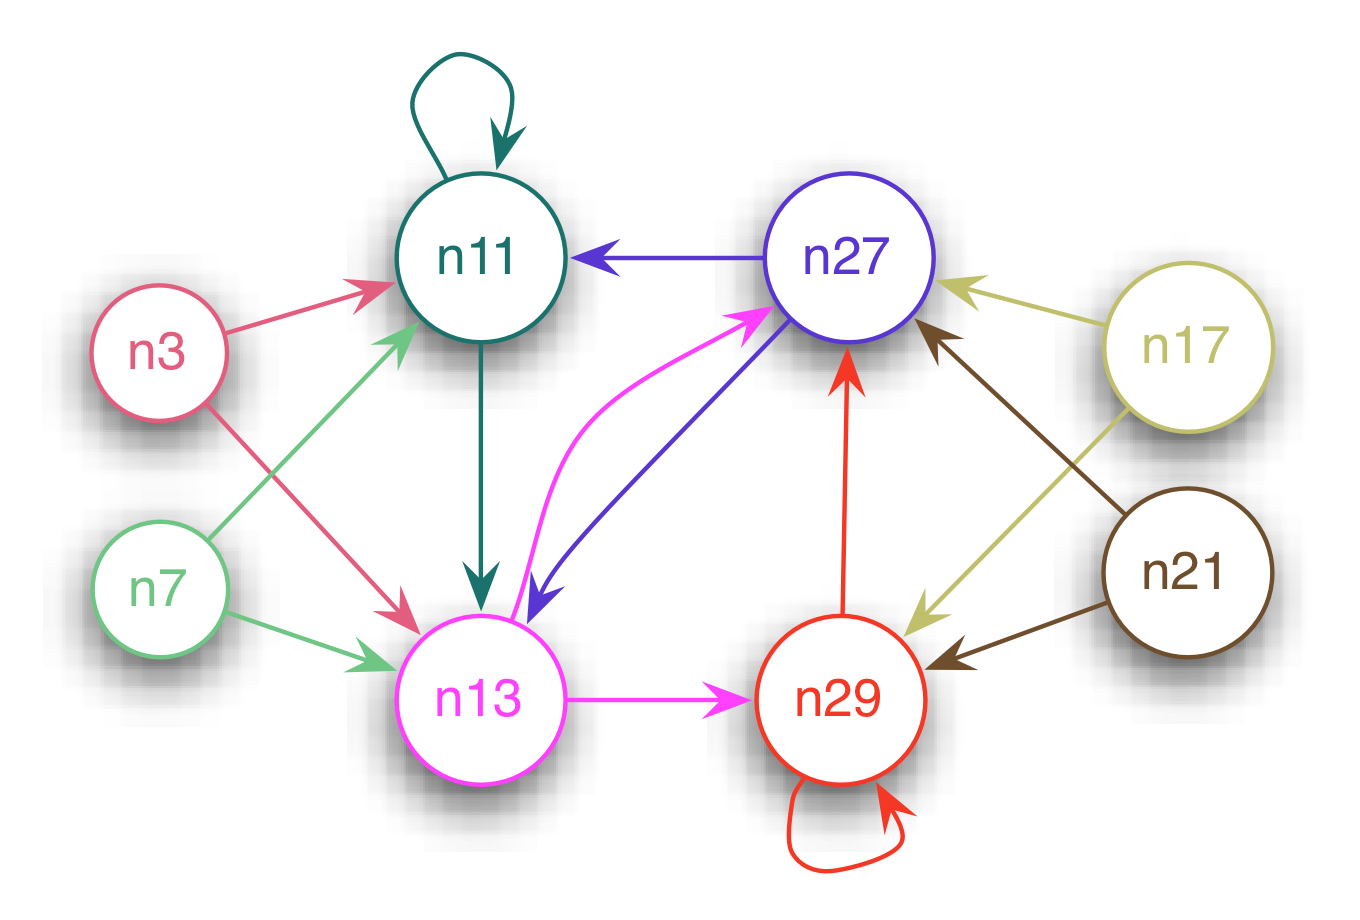
\includegraphics{example_scc.png}
\caption{SCC subgraph generated.}\end{figure}

\begin{notice}{note}{Note:}
To generate all the SCCs of a graph we use the \href{https://github.com/bwesterb/py-tarjan/}{Tarjan's Algorithm}.
\end{notice}


\strong{See Also:}


{\hyperref[modelCheckingGraph:modelCheckingGraph.getModelCheckingAtoms]{\code{modelCheckingGraph.getModelCheckingAtoms()}}}, {\hyperref[modelCheckingGraph:modelCheckingGraph.getModelCheckingGraph]{\code{modelCheckingGraph.getModelCheckingGraph()}}} 



\end{fulllineitems}

\index{initialNodesEntailFormula() (in module searchingAlgorithm)}

\begin{fulllineitems}
\phantomsection\label{searchingAlgorithm:searchingAlgorithm.initialNodesEntailFormula}\pysiglinewithargsret{\code{searchingAlgorithm.}\bfcode{initialNodesEntailFormula}}{\emph{scc\_graph}, \emph{initial\_nodes}, \emph{model\_checking\_atoms}, \emph{formula}}{}
Checks if the initial nodes of a model checking graph satisfy a temporal formula.
\begin{quote}\begin{description}
\item[{Parameters}] \leavevmode\begin{itemize}
\item {} 
\textbf{scc\_graph} -- 

\item {} 
\textbf{initial\_nodes} -- 

\item {} 
\textbf{model\_checking\_atoms} -- 

\item {} 
\textbf{formula} -- 

\end{itemize}

\item[{Returns}] \leavevmode


\item[{Return type}] \leavevmode
Boolean.

\item[{Example }] \leavevmode
\end{description}\end{quote}

\end{fulllineitems}

\index{isSatisfied() (in module searchingAlgorithm)}

\begin{fulllineitems}
\phantomsection\label{searchingAlgorithm:searchingAlgorithm.isSatisfied}\pysiglinewithargsret{\code{searchingAlgorithm.}\bfcode{isSatisfied}}{\emph{formula}, \emph{tcc\_structure}, \emph{model\_checking\_atoms}, \emph{model\_checking\_scc\_subgraphs}}{}
\end{fulllineitems}

\index{isSelfFulfilling() (in module searchingAlgorithm)}

\begin{fulllineitems}
\phantomsection\label{searchingAlgorithm:searchingAlgorithm.isSelfFulfilling}\pysiglinewithargsret{\code{searchingAlgorithm.}\bfcode{isSelfFulfilling}}{\emph{scc\_graph}, \emph{initial\_nodes}, \emph{model\_checking\_atoms}}{}
Checks if a SCC graph is a self-fulfilling SCC graph.
\begin{quote}\begin{description}
\item[{Parameters}] \leavevmode\begin{itemize}
\item {} 
\textbf{scc\_graph} (\emph{Dictionary}) -- SCC graph

\item {} 
\textbf{initial\_nodes} (\emph{List}) -- List of initial nodes of the model checking graph.

\item {} 
\textbf{model\_checking\_atoms} (\emph{List of atoms.}) -- Model checking atoms

\end{itemize}

\item[{Returns}] \leavevmode
\code{True} if the graph is a self-fulfilling SCC or \code{False} otherwise.

\item[{Return type}] \leavevmode
Boolean

\item[{Example }] \leavevmode
\end{description}\end{quote}

\begin{Verbatim}[commandchars=\\\{\}]
\PYG{g+gp}{\PYGZgt{}\PYGZgt{}\PYGZgt{} }\PYG{k+kn}{from} \PYG{n+nn}{searchingAlgorithm} \PYG{k+kn}{import} \PYG{o}{*}
\PYG{g+gp}{\PYGZgt{}\PYGZgt{}\PYGZgt{} }\PYG{n}{sccGraph} \PYG{o}{=} \PYG{p}{\PYGZob{}}\PYG{l+m+mi}{3}\PYG{p}{:} \PYG{p}{[}\PYG{l+m+mi}{11}\PYG{p}{,} \PYG{l+m+mi}{13}\PYG{p}{]}\PYG{p}{,} \PYG{l+m+mi}{7}\PYG{p}{:} \PYG{p}{[}\PYG{l+m+mi}{11}\PYG{p}{,} \PYG{l+m+mi}{13}\PYG{p}{]}\PYG{p}{,} \PYG{l+m+mi}{11}\PYG{p}{:} \PYG{p}{[}\PYG{l+m+mi}{11}\PYG{p}{,} \PYG{l+m+mi}{13}\PYG{p}{]}\PYG{p}{,} \PYG{l+m+mi}{13}\PYG{p}{:} \PYG{p}{[}\PYG{l+m+mi}{27}\PYG{p}{,} \PYG{l+m+mi}{29}\PYG{p}{]}\PYG{p}{,} \PYG{l+m+mi}{17}\PYG{p}{:} \PYG{p}{[}\PYG{l+m+mi}{27}\PYG{p}{,} \PYG{l+m+mi}{29}\PYG{p}{]}\PYG{p}{,} \PYG{l+m+mi}{21}\PYG{p}{:} \PYG{p}{[}\PYG{l+m+mi}{27}\PYG{p}{,} \PYG{l+m+mi}{29}\PYG{p}{]}\PYG{p}{,} \PYG{l+m+mi}{27}\PYG{p}{:} \PYG{p}{[}\PYG{l+m+mi}{11}\PYG{p}{,} \PYG{l+m+mi}{13}\PYG{p}{]}\PYG{p}{,} \PYG{l+m+mi}{29}\PYG{p}{:} \PYG{p}{[}\PYG{l+m+mi}{27}\PYG{p}{,} \PYG{l+m+mi}{29}\PYG{p}{]}\PYG{p}{\PYGZcb{}}
\PYG{g+gp}{\PYGZgt{}\PYGZgt{}\PYGZgt{} }\PYG{n}{initialNodes} \PYG{o}{=} \PYG{p}{[}\PYG{l+m+mi}{1}\PYG{p}{,} \PYG{l+m+mi}{2}\PYG{p}{,} \PYG{l+m+mi}{3}\PYG{p}{,} \PYG{l+m+mi}{4}\PYG{p}{,} \PYG{l+m+mi}{5}\PYG{p}{,} \PYG{l+m+mi}{6}\PYG{p}{,} \PYG{l+m+mi}{7}\PYG{p}{,} \PYG{l+m+mi}{8}\PYG{p}{,} \PYG{l+m+mi}{17}\PYG{p}{,} \PYG{l+m+mi}{18}\PYG{p}{,} \PYG{l+m+mi}{19}\PYG{p}{,} \PYG{l+m+mi}{20}\PYG{p}{,} \PYG{l+m+mi}{21}\PYG{p}{,} \PYG{l+m+mi}{22}\PYG{p}{,} \PYG{l+m+mi}{23}\PYG{p}{,} \PYG{l+m+mi}{24}\PYG{p}{]}
\PYG{g+gp}{\PYGZgt{}\PYGZgt{}\PYGZgt{} }\PYG{n}{isSelfFulfilling}\PYG{p}{(}\PYG{n}{sccGraph}\PYG{p}{,} \PYG{n}{initialNodes}\PYG{p}{,} \PYG{n}{model\PYGZus{}checking\PYGZus{}atoms}\PYG{p}{)}
\PYG{g+go}{True}
\end{Verbatim}


\strong{See Also:}


{\hyperref[modelCheckingGraph:modelCheckingGraph.getModelCheckingAtoms]{\code{modelCheckingGraph.getModelCheckingAtoms()}}}, {\hyperref[searchingAlgorithm:searchingAlgorithm.getModelCheckingSCCSubgraphs]{\code{getModelCheckingSCCSubgraphs()}}}, {\hyperref[searchingAlgorithm:searchingAlgorithm.getInitialNodes]{\code{getInitialNodes()}}}



\end{fulllineitems}



\chapter{Indices and tables}
\label{index:indices-and-tables}\begin{itemize}
\item {} 
\emph{genindex}

\item {} 
\emph{modindex}

\item {} 
\emph{search}

\end{itemize}

\begin{thebibliography}{MP95}
\bibitem[MP95]{MP95}{\phantomsection\label{modelCheckingGraph:mp95} 
Zohar Manna and Amir Pnueli. Temporal Verification of Reactive Systems: Safety. Springer-Verlag New York, Inc., 1995.
}
\end{thebibliography}


\renewcommand{\indexname}{Python Module Index}
\begin{theindex}
\def\bigletter#1{{\Large\sffamily#1}\nopagebreak\vspace{1mm}}
\bigletter{c}
\item {\texttt{closure}}, \pageref{closure:module-closure}
\indexspace
\bigletter{f}
\item {\texttt{formula}}, \pageref{formula:module-formula}
\indexspace
\bigletter{m}
\item {\texttt{modelCheckingGraph}}, \pageref{modelCheckingGraph:module-modelCheckingGraph}
\indexspace
\bigletter{s}
\item {\texttt{searchingAlgorithm}}, \pageref{searchingAlgorithm:module-searchingAlgorithm}
\end{theindex}

\renewcommand{\indexname}{Index}
\printindex
\end{document}
